\documentclass[9pt,professionalfont,t,aspectratio=169]{beamer}
\usepackage{amsmath}
\usepackage{amssymb}
\usepackage{amsthm}
\usepackage{empheq}
\usepackage{xparse}
\usepackage[export]{adjustbox}
\usepackage{varwidth}
\usepackage{tabulary}
\usepackage{xcolor}
\usepackage{hhline}
\usepackage{relsize}
\usepackage{framed}
\usepackage[beamer]{hf-tikz}
\usepackage{multirow}

\usepackage[style=authoryear]{biblatex}
\usepackage{bm}
\usepackage{changepage}
\usepackage[T1]{fontenc}
\usepackage{concmath}
\usepackage{mathrsfs}
\usepackage{mathtools}
\usepackage[thinlines]{easytable}
\usepackage{xy}
\usepackage{wrapfig}
\usepackage{pgfplots,tikz}
\usepackage{soul}
\usepackage{verbatim}
\usetikzlibrary{matrix,positioning,arrows}
\usetikzlibrary{tikzmark}
\usetikzlibrary{fit}
\usetheme[progressbar=frametitle]{metropolis}
\usepackage{appendixnumberbeamer}
\usepackage{ wasysym }

\usepackage{booktabs}
%\usepackage[scale=2]{ccicons}
\usepackage{lmodern}
\usepackage{xspace}
\usepackage{graphicx}
\usepackage{mathtools}
\usepackage{float}
\usepackage{amstext}
\usepackage{array}
\usepackage{lipsum}
\usepackage{amsfonts}              
\usepackage{amsthm}               
\usepackage{amssymb}
%\usepackage{multimedia}
\usepackage{media9}
\usepackage[absolute,overlay]{textpos}
\usepackage[font=small]{caption}
\captionsetup[figure]{labelformat=empty}%
\captionsetup[table]{labelformat=empty}%
\usepackage{pgfplots,tikz}
\usepackage{soul}
\usepackage{verbatim}
\usetikzlibrary{matrix,positioning,arrows}
\usetikzlibrary{tikzmark}
\usetikzlibrary{fit}


\DeclareMathOperator{\Avg}{\mathbb{E}}

\newcommand*\numcircledmod[1]{\raisebox{.5pt}{\textcircled{\raisebox{-.9pt} {#1}}}}

%\usepackage{animate}
\usepackage{etoolbox}% http://ctan.org/pkg/etoolbox

\setbeamercolor{block title}{fg=Medalist,bg=white} % Colors of the block titles

\setbeamercolor{block body}{fg=black,bg=white} % Colors of the body of blocks

\setbeamercolor{block alerted title}{fg=white,bg=BerkBlue!80} % Colors of the highlighted block titles

\setbeamercolor{block alerted body}{fg=black,bg=BerkBlue!10} % Colors of the body of highlighted blocks

\setbeamercolor{block title example}{fg=BerkBlue,bg=white} % Colors of the block titles

\setbeamercolor{block body example}{fg=black,bg=white} % Colors of the body of blocks

\setbeamertemplate{caption}{\raggedright\insertcaption\par}

\newcommand\setItemnumber[1]{\setcounter{enumi}{\numexpr#1-1\relax}}

\newcommand{\ch}[1]{{\color{purple}#1}}
\newcommand{\km}[1]{{\color{red}#1}}
\newcommand{\ed}[1]{{\color{blue}#1}}

\newbox\FBox
\NewDocumentCommand\Highlight{O{black}O{white}mO{0.5pt}O{0pt}O{0pt}}{%
    \setlength\fboxsep{#4}\sbox\FBox{\fcolorbox{#1}{#2}{#3\rule[-#5]{0pt}{#6}}}\usebox\FBox}
      
\DeclareCiteCommand{\longcite}{}{%
    \printnames{author}, \printfield{journaltitle} \printfield{year}}{;}{}%
    

\newcommand*\diff{\mathop{}\!\mathrm{d}}
\newcommand*\Diff[1]{\mathop{}\!\mathrm{d^#1}}
\def\*#1{\mathbf{#1}}
\DeclareMathOperator{\Tr}{Tr}

% Syntax: \colorboxed[<color model>]{<color specification>}{<math formula>}
\newcommand*{\colorboxed}{}
\def\colorboxed#1#{%
  \colorboxedAux{#1}%
}
\newcommand*{\colorboxedAux}[3]{%
  % #1: optional argument for color model
  % #2: color specification
  % #3: formula
  \begingroup
    \colorlet{cb@saved}{.}%
    \color#1{#2}%
    \boxed{%
      \color{cb@saved}%
      #3%
    }%
  \endgroup
}

\title{Excitations, Emergent Facilitation and Glassy Dynamics in Supercooled Liquids}
% \date{Virtual Seminar --  Theory Club, \today}
\date{APS March Meeting 2024, March 4, 2024}
\author{Muhammad R. Hasyim\inst{1}, Kranthi K. Mandadapu\inst{2}}
\institute[Affiliations]{
    \inst{1}%
    Department of Chemical and Biomolecular Engineering, University of California, Berkeley, CA 94720
    
    \inst{2}%
    Chemical Division, Lawrence Berkeley National Laboratory, Berkeley, CA 94720
%    \\ 
%    Contact: \url{mh7373@nyu.edu}
}
% \newcommand\FrameText[1]{%
% \begin{textblock*}{\paperwidth}(\textwidth-\widthof{#1},0.92\textheight)\raggedright #1\hspace{0.5em}
% \end{textblock*}}
\metroset{block=fill}
\begin{document}

\maketitle 

% Part A: Introduction & Framework
\begin{frame}[c]\label{a.1}
\frametitle{Supercooled Liquids a Glance}%: Why Study Supercooled Liquids?}%at is a Supercooled Liquid?}
\vspace{-12.0pt}
\begin{overprint}
\onslide<1-5>\begin{block}{\large \centering Why Study Supercooled Liquids?}
\vspace{6pt}
\centering A supercooled liquid contradicts our intuition on how \only<2->{slow (\textbf{glassy}) }dynamics relates to structure.
\end{block}
%\vspace{-4pt}}
\onslide<6->
\begin{block}{\large \centering Central Question}
\vspace{6pt}
\centering How to understand the dramatic slowdown and dynamical heterogeneity of supercooled liquids?
\end{block}
\end{overprint}
%
%\vspace{4pt}
\begin{columns}
\begin{column}{0.5\textwidth}
\centering  \uncover<2->{\textbf{\large Dynamics}}

\begin{figure}[t]

\begin{overprint}
\onslide<2>\centering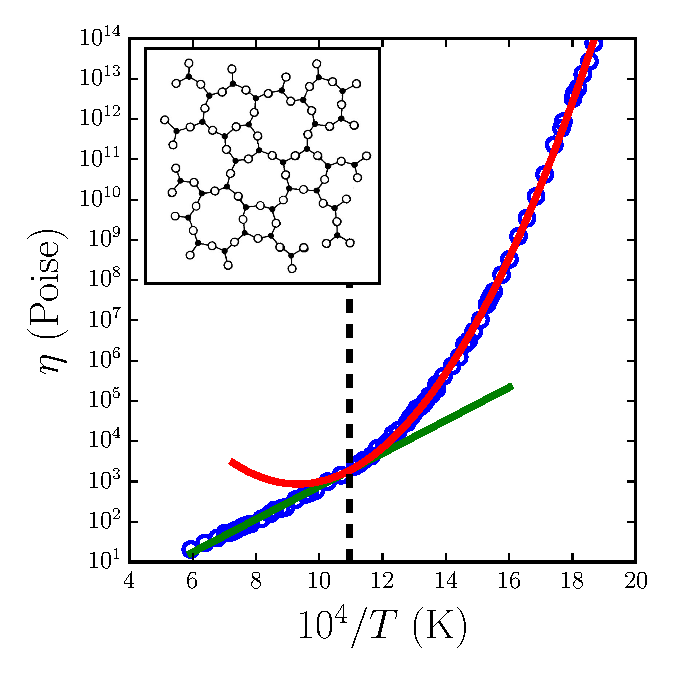
\includegraphics[height=0.6\textheight]{intro_glassy/timerelax_b2o3_4.pdf}
\caption{Viscosity of boron oxide ($\mathrm{B_2 O_3}$) (Tweer, Simmons, and Macedo, \textit{J. Chem. Phys.},  1970).}

\onslide<3>\centering\includegraphics[height=0.6\textheight]{a.3-intro_dh/softspots_220.png}
\caption{\textbf{Dynamical heterogeneity}: localized mobile regions (at early times) that spread over time.}  

\onslide<4->\centering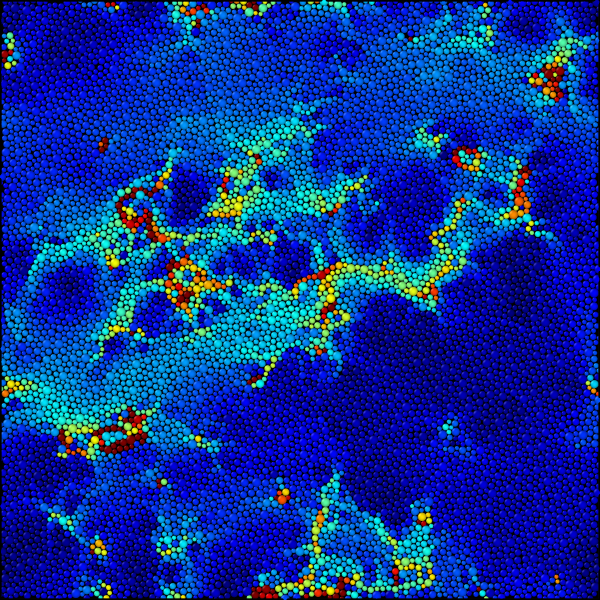
\includegraphics[height=0.6\textheight]{intro_glassy/softspots_280.png}
\caption{\textbf{Dynamical heterogeneity}: localized mobile regions (at early times) that spread over time.}  
\end{overprint}

\end{figure}



% \only<4->
% {
% \begin{figure}[t]
% \centering
% 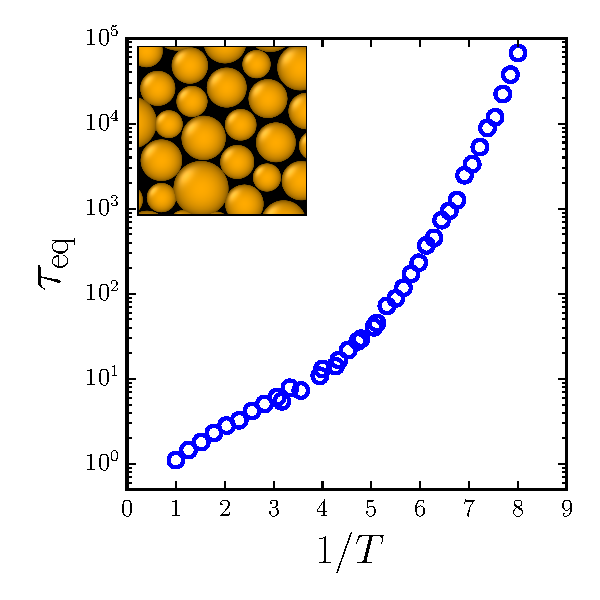
\includegraphics[height=0.6\textheight]{figures/timerelax_poly12_1.pdf}
% \caption{\textbf{Super-Arrhenius: }Dramatic slowdown at temperatures $T$ below onset temperature $T_\mathrm{o}$ (dashed line).}
% \end{figure}
% }

% \only<7->{
% \begin{figure}[t]
% \includegraphics[height=0.73\textheight]{figures/facilitation.png}
% \caption{2D 50:50 Binary Lennard-Jones system, showing the coordinated movement of particles (Keys et.al. 1, 021013, \textit{Phys. Rev. X}, 2011).} 
% \end{figure}
% }

\end{column}

\begin{column}{0.5\textwidth}
\centering  \uncover<5->{\textbf{\large Structure}}


\begin{figure}[t]
\begin{overprint}
\onslide<5>\centering\includegraphics[height=0.6\textheight]{a.3-intro_dh/poly12_lowT.png}\caption{It is not obvious from the structure where the heterogeneity is coming from!}
\onslide<6->\centering\includegraphics[height=0.6\textheight]{a.3-intro_dh/gr_poly12_single-1.pdf}
\caption{Radial distribution function (RDF). Data sweeps across \textbf{4 decades in relaxation time}.}

% (it is disordered and well-dispersed)!}% structure of supercooled liquids is disordered and homogeneous at all temperatures}
\end{overprint}

%Locations of the peaks in the radial distribution function (RDF) remains the same, despite dramatic slowdown in dynamics.}
\end{figure}


% \only<6->{
% \begin{figure}[t]
% \centering
% \uncover<7->{\includegraphics[height=0.6\textheight]{figures/gr_poly12_single.pdf}}
% \caption{Local structure (from the RDF) remains qualitatively same under a wide range of supercooled conditions.}
% \end{figure}
% }

\end{column}
\end{columns}
\end{frame} 
\begin{frame}[t]\label{a.2}
\frametitle{A Dynamics-Based Perspective: Dynamical Facilitation Theory}

DF theory (Chandler and Garrahan, \textit{Annu. Rev. Phys. Chem}, 2010) can explain glassy dynamics \textbf{without knowledge of local structure} with two key ideas:


% \only<5->
% {
% \begin{block}{\centering Highlights of DF Theory}
% \uncover<6->{Requires no knowledge of local structure or static properties.} \uncover<7->{Guided by kinetically-constrained lattice models, e.g., the Arrow model (Garrahan and Chandler, \textit{PNAS}, (2003)), to make predictions.}
% %, that captures the idea of facilitating excitations. }
% \end{block}
% }%\vspace{9pt}

\begin{columns}[T]
\begin{column}[T]{0.5\textwidth}

\onslide<2->\centering\textbf{\Large Excitations}

\begin{figure}[t]
\begin{overprint}

\onslide<2>\centering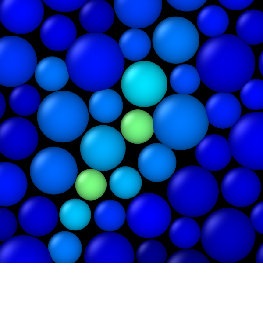
\includegraphics[height=0.525\textheight]{2.a-intro_dftheory/DF_Theory_Excitations_Zoom_0.pdf}\caption{Below the onset temperature $T_\mathrm{o}$, localized excitations drive glassy dynamics! (Keys, et al. \textit{Phys. Rev. X} 2011)}

\onslide<3>\centering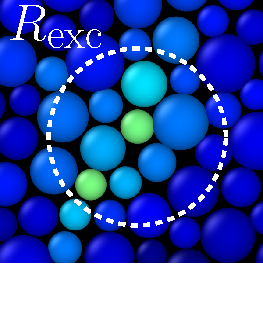
\includegraphics[height=0.525\textheight]{2.a-intro_dftheory/DF_Theory_Excitations_Zoom_1.pdf}\caption{Below the onset temperature $T_\mathrm{o}$, localized excitations drive glassy dynamics! (Keys, et al. \textit{Phys. Rev. X} 2011)}

\onslide<4->\centering\includegraphics[height=0.525\textheight]{2.a-intro_dftheory/DF_Theory_Excitations_Zoom_2.pdf}\caption{Below the onset temperature $T_\mathrm{o}$, localized excitations drive glassy dynamics! (Keys, et al. \textit{Phys. Rev. X} 2011)}


\end{overprint}
\end{figure}

\end{column}
%\vrule{}
\begin{column}[T]{0.50\textwidth}

\onslide<5->\centering\textbf{\Large Facilitation}
\begin{figure}[t]
\begin{center}
\begin{overprint}
\onslide<5>\centerline{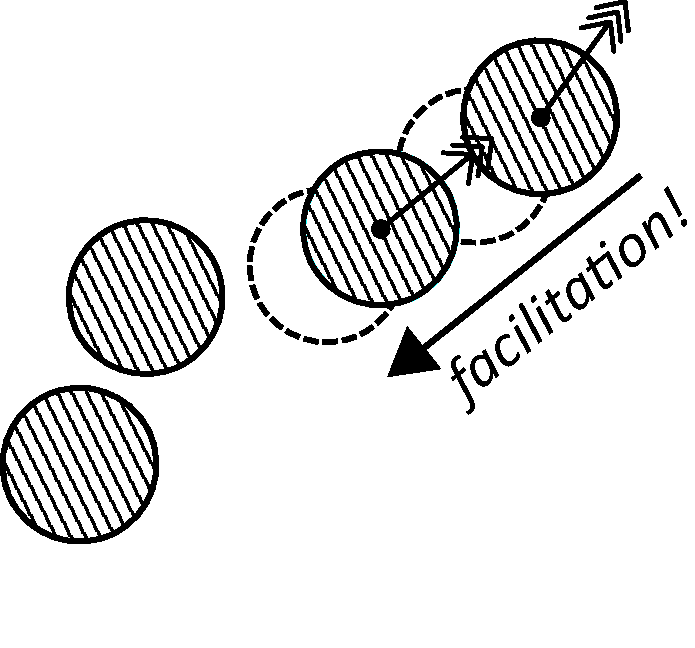
\includegraphics[height=0.525\textheight]{2.a-intro_dftheory/facilitation_closer_1.pdf}}
\onslide<6->\centerline{\includegraphics[height=0.525\textheight]{2.a-intro_dftheory/facilitation_closer_2.pdf}}
\end{overprint}
\end{center}
\caption{Excitations facilitate the creation and relaxation of another excitation close by.}
\end{figure}

\end{column}
\end{columns}

\end{frame}
\begin{frame}\label{a.3}
\frametitle{Elastic Dynamical Facilitation (EDF) Theory: The Complete Picture}

EDF theory unifies elasticity with glassy dynamics through \textbf{three interconnected pillars} that provide a complete microscopic framework:

\vspace{0.5em}

\begin{columns}[T]
\begin{column}[T]{0.33\textwidth}

\centering\textbf{\Large Excitations}

\begin{figure}[t]
\centering\includegraphics[height=0.45\textheight]{a.2-intro_dftheory/DF_Theory_Excitations_Zoom_2.pdf}
\caption{\textbf{Pure shear excitations} with energy scale $J_\sigma \sim G R_\mathrm{exc}^2 \epsilon_\mathrm{c}^2$}
\end{figure}

\end{column}

\begin{column}[T]{0.33\textwidth}

\centering\textbf{\Large Onset Temperature}

\begin{figure}[t]
\begin{center}
\centerline{\includegraphics[height=0.45\textheight]{c.1-kt_msdintro/msd-supercooledliq-5.pdf}}
\end{center}
\caption{\textbf{2D melting theory} explains $T_\mathrm{o}$ from elastic stability}
\end{figure}

\end{column}

\begin{column}[T]{0.33\textwidth}

\centering\textbf{\Large Facilitation}

\begin{figure}[t]
\begin{center}
\centerline{\includegraphics[height=0.45\textheight]{a.2-intro_dftheory/facilitation_closer_2.pdf}}
\end{center}
\caption{\textbf{Elastic stress fields} create emergent facilitation}
\end{figure}

\end{column}
\end{columns}

\vspace{1em}

\begin{block}{\centering Key Insight}
\centering \textbf{Elasticity} provides the microscopic foundation for all three pillars, creating a \textbf{unified quantitative theory}: 
$$\boxed{\text{EDF Theory} = \text{Elastic Excitations} + \text{Elastic Onset} + \text{Elastic Facilitation}}$$
\end{block}

\end{frame} 

% Part B: Excitations Theory
\begin{frame}[c]\label{b.1}
\frametitle{A Theory of Localized Excitations: Pure Shear Excitations}

\vspace{-0.5em}
\begin{block}{\centering \large Origin of Excitations }
\centering The inherent \textbf{structure and elasticity (solid-like)} of supercooled liquids $\leftrightarrow$ localized excitations! {\footnotesize (Hasyim, Mandadapu,  \textit{J. Chem. Phys.} 155, 044504 2021)}
\end{block}
\vspace{-0.5em}
\begin{columns}[T]
\begin{column}[T]{0.4\textwidth}

\begin{figure}[t]

\begin{overprint}
\onslide<2>\centering\includegraphics[width=1.1\linewidth]{5.c-fac_summodel/PEL.pdf}\caption{Glassy dynamics is hopping between energy minima (inherent states)  (Stillinger and Weber, \textit{Phys. Rev. A} 1982)}

\onslide<3>\centering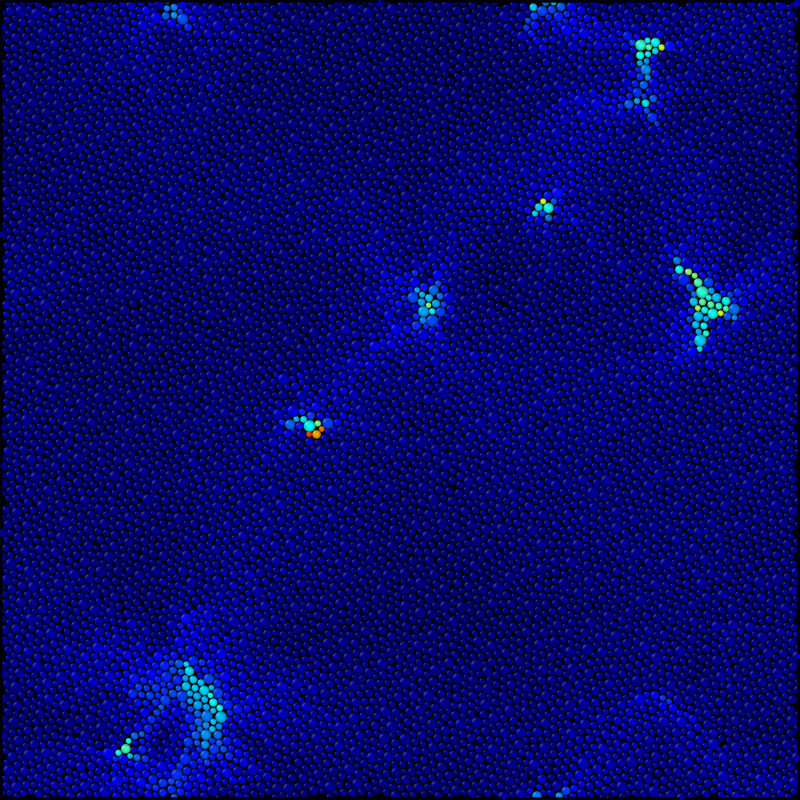
\includegraphics[width=0.85\linewidth]{1.b-exc_pureshear/zoomout_dispmag.png}\caption{Excitations of a model glass former, detected by the initial dynamic heterogeneity.}

\onslide<4>\centering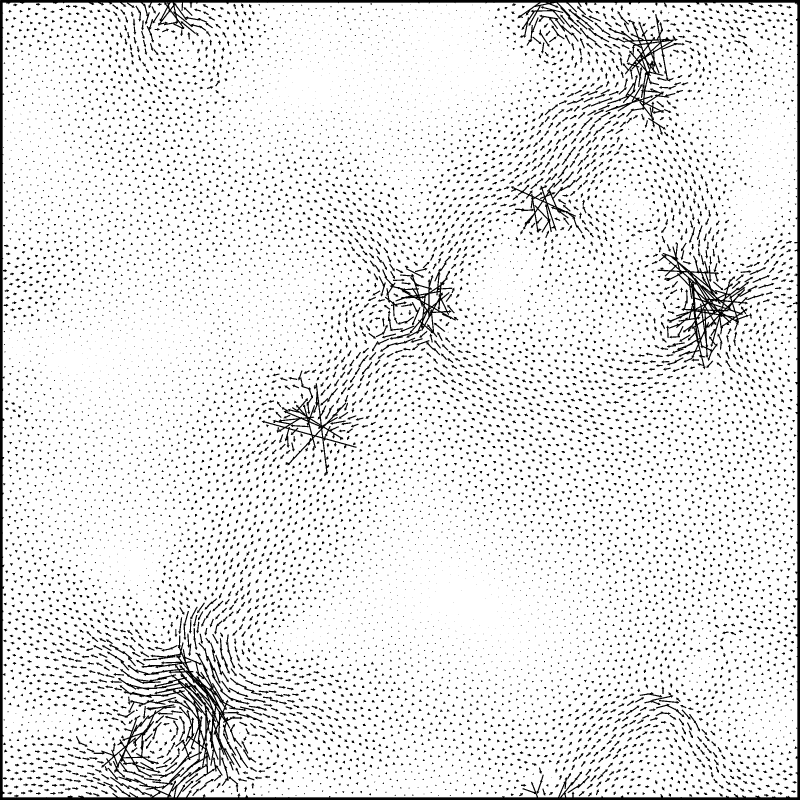
\includegraphics[width=0.85\linewidth]{1.b-exc_pureshear/zoomout_dispvector.png}\caption{The displacement vector field due to excitations in the liquid.}

\onslide<5>\centering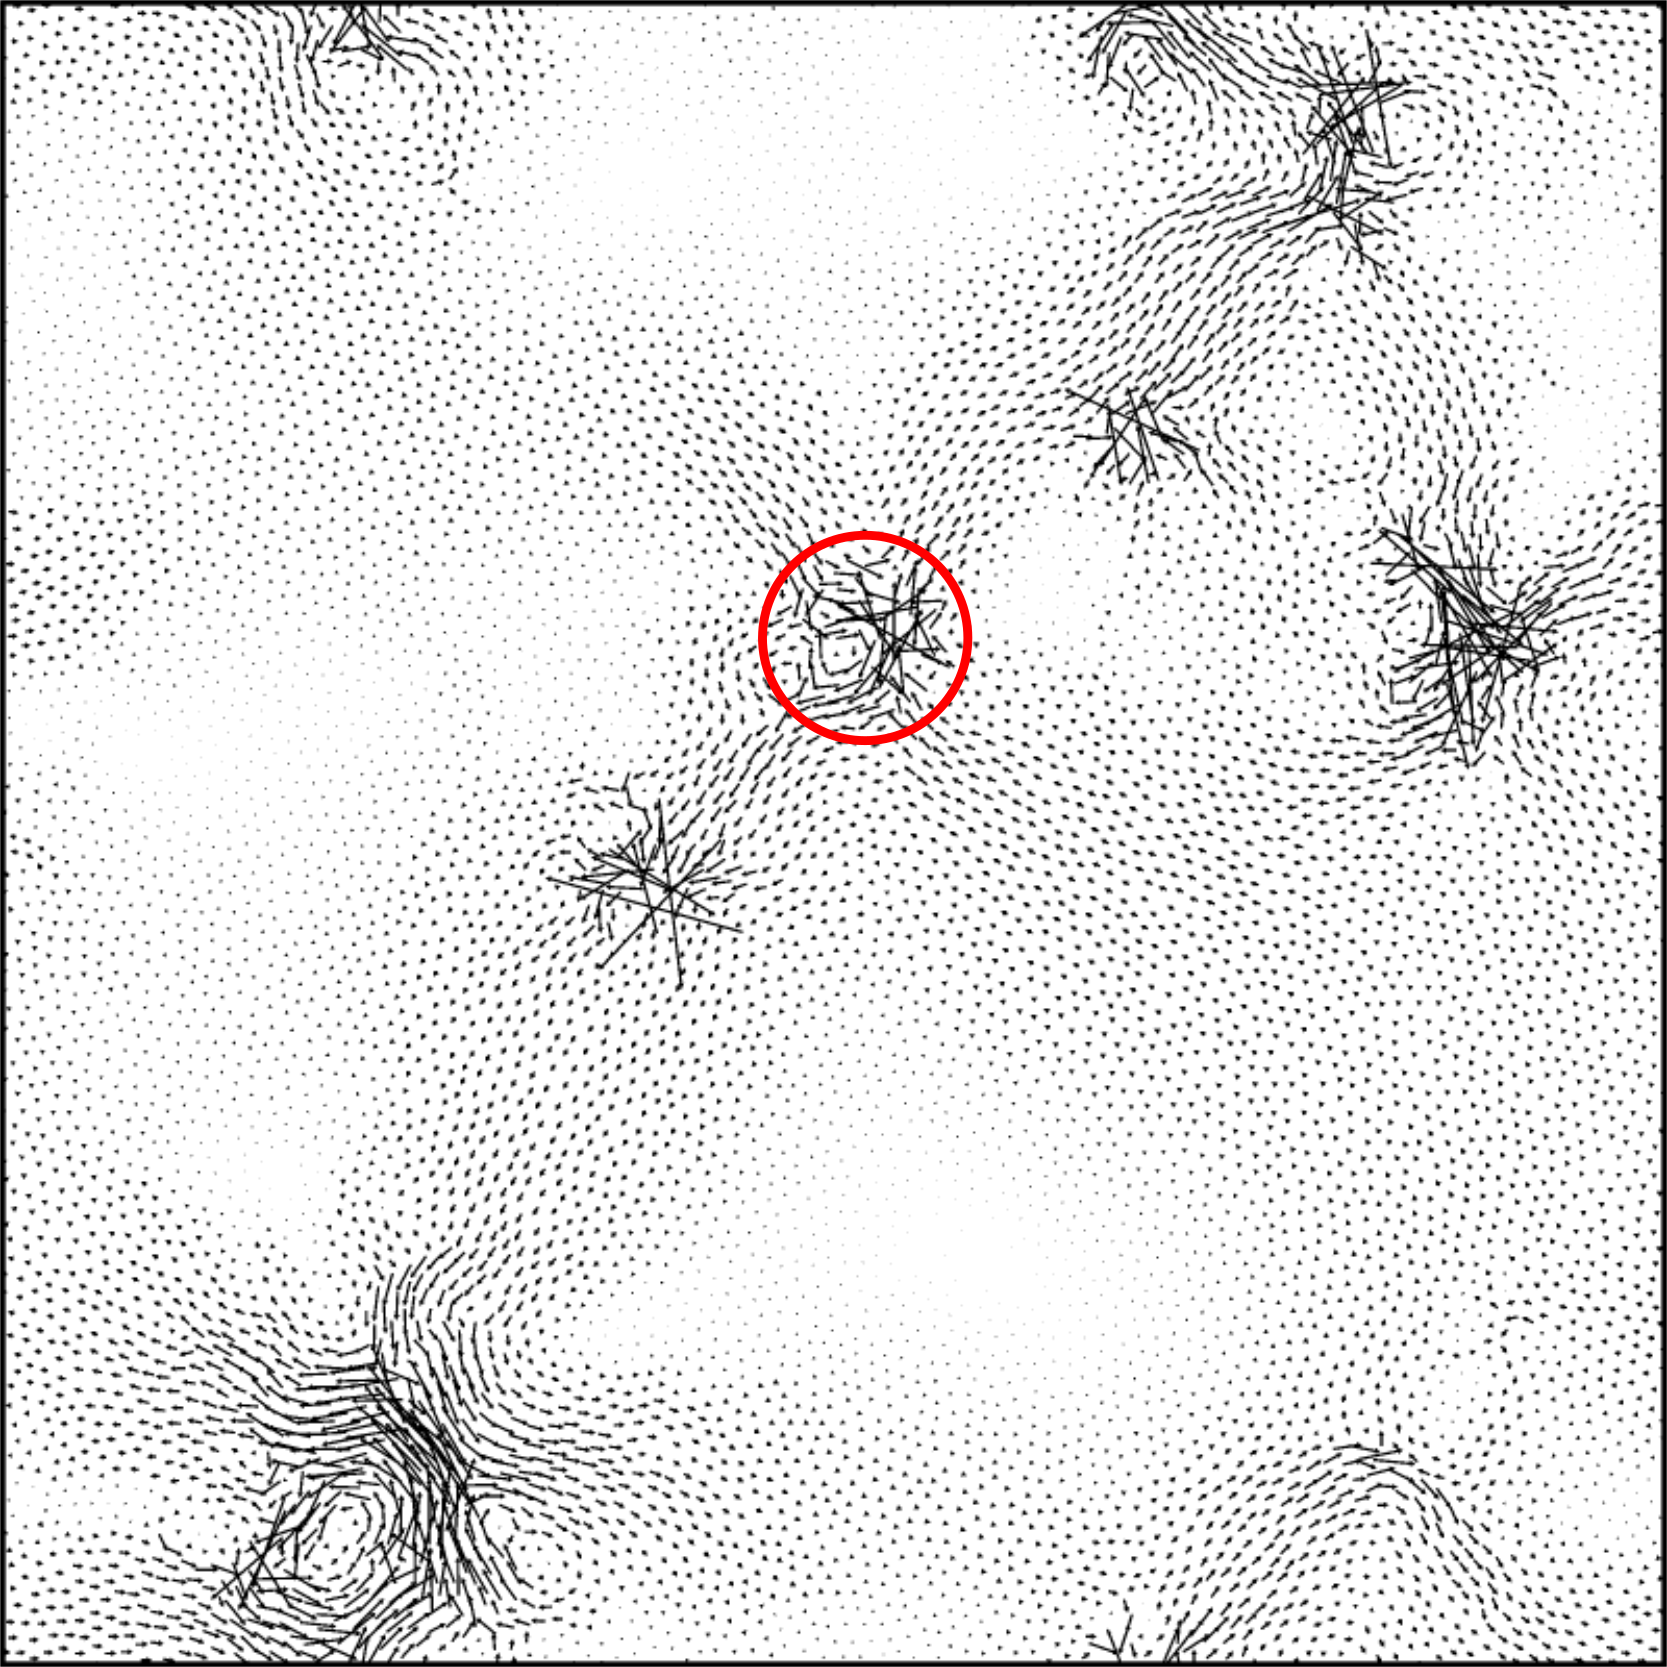
\includegraphics[width=0.85\linewidth]{1.b-exc_pureshear/zoomout_dispvector_1.png}\caption{The displacement field vector field due to excitations in the liquid.}

\onslide<6>\centering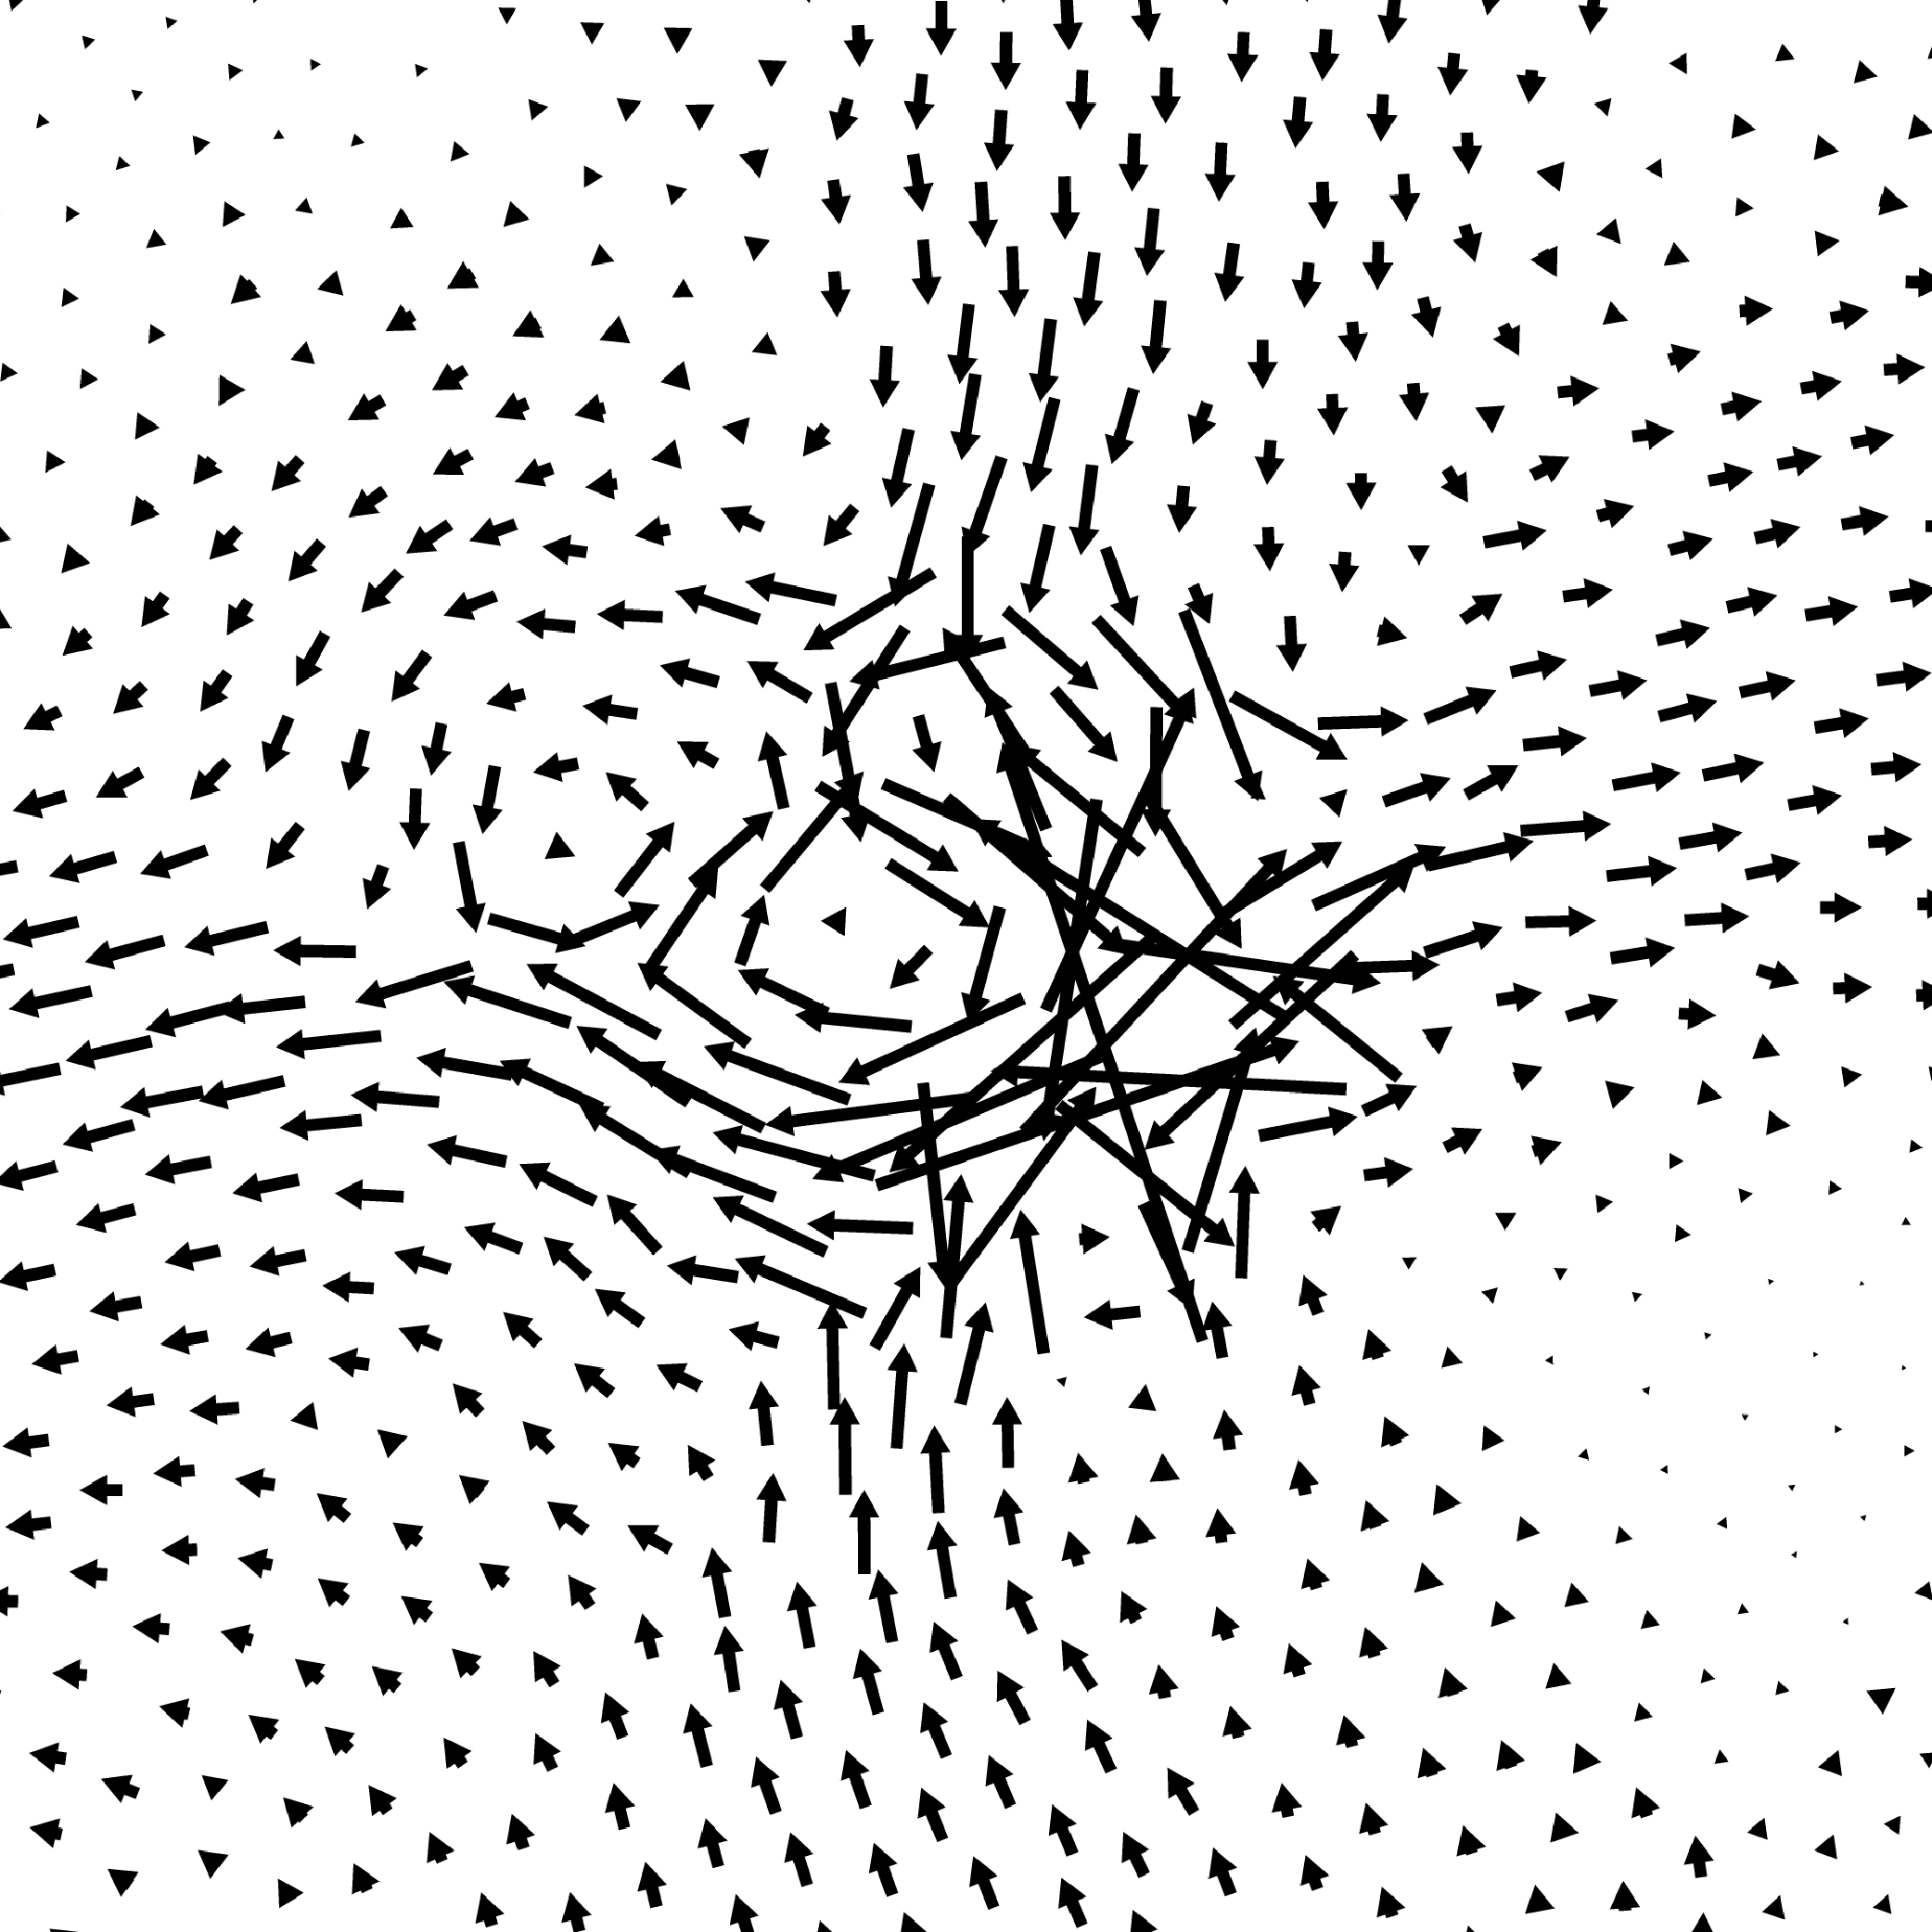
\includegraphics[width=0.85\linewidth]{1.b-exc_pureshear/zoomin-0.pdf}\caption{An excitation reorganizes the surrounding solid medium.}

\onslide<7>\centering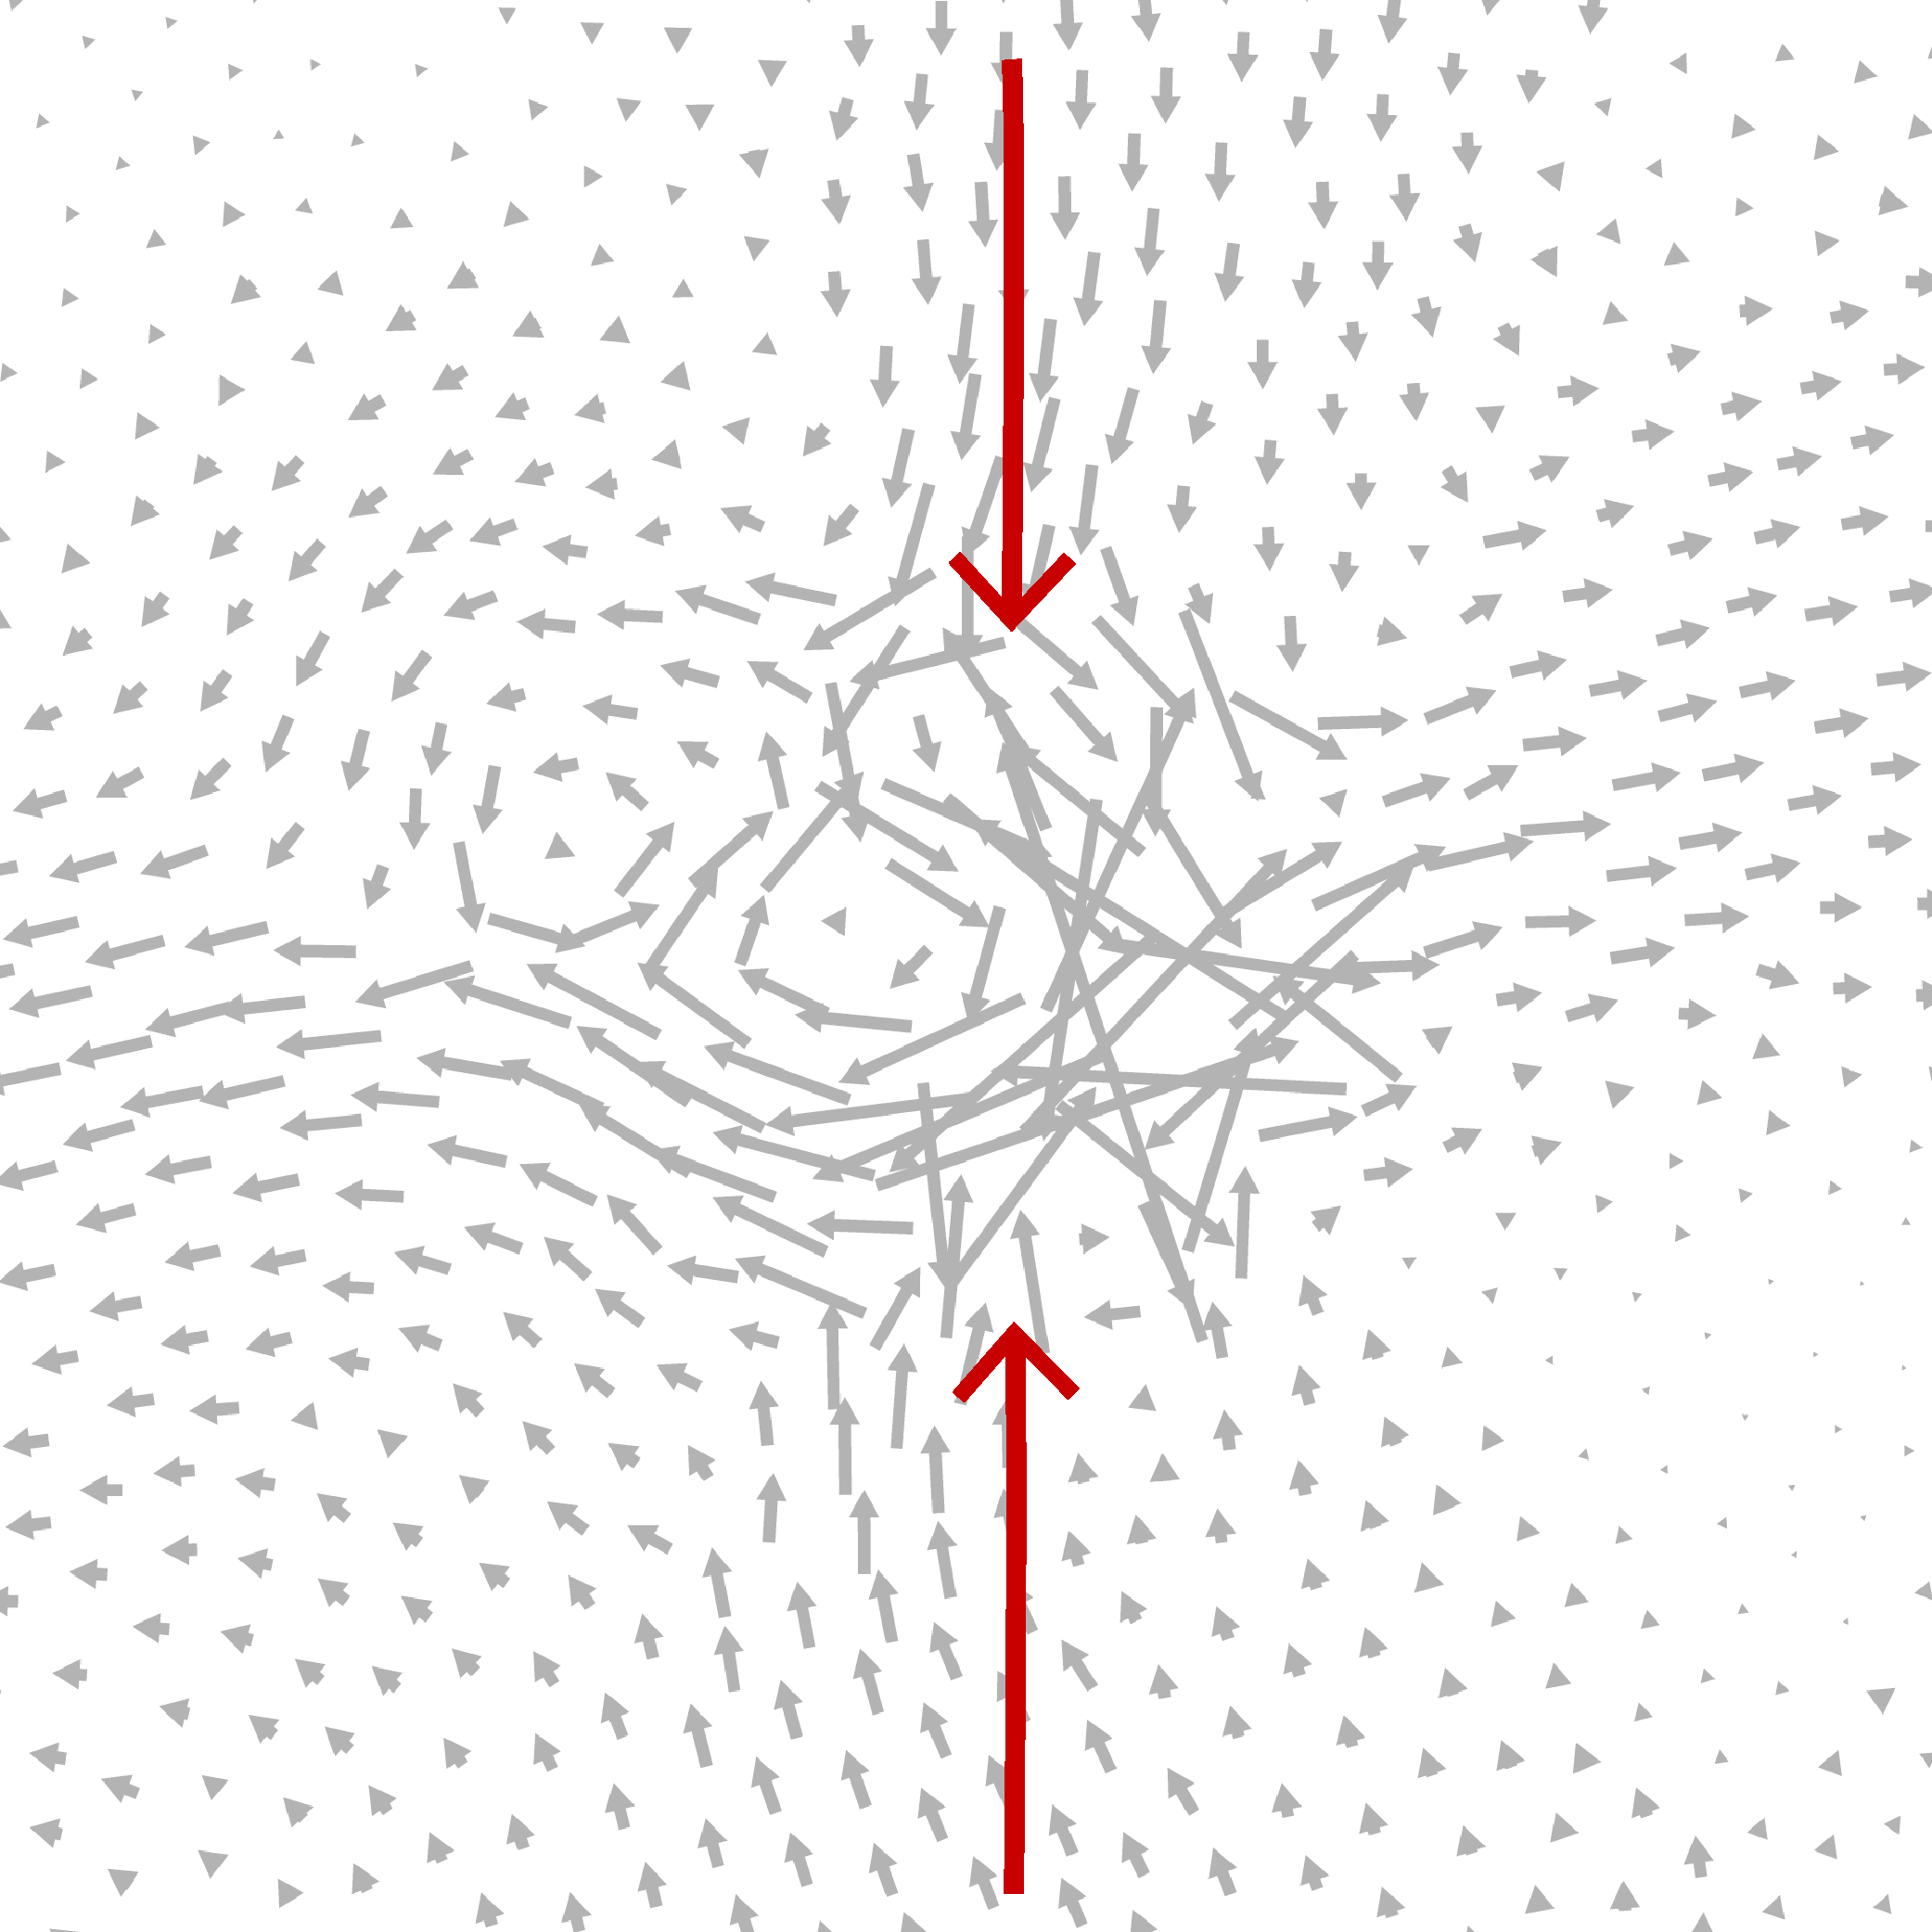
\includegraphics[width=0.85\linewidth]{1.b-exc_pureshear/zoomin-1.pdf}\caption{In one axis, there's compressive flow.}

\onslide<8>\centering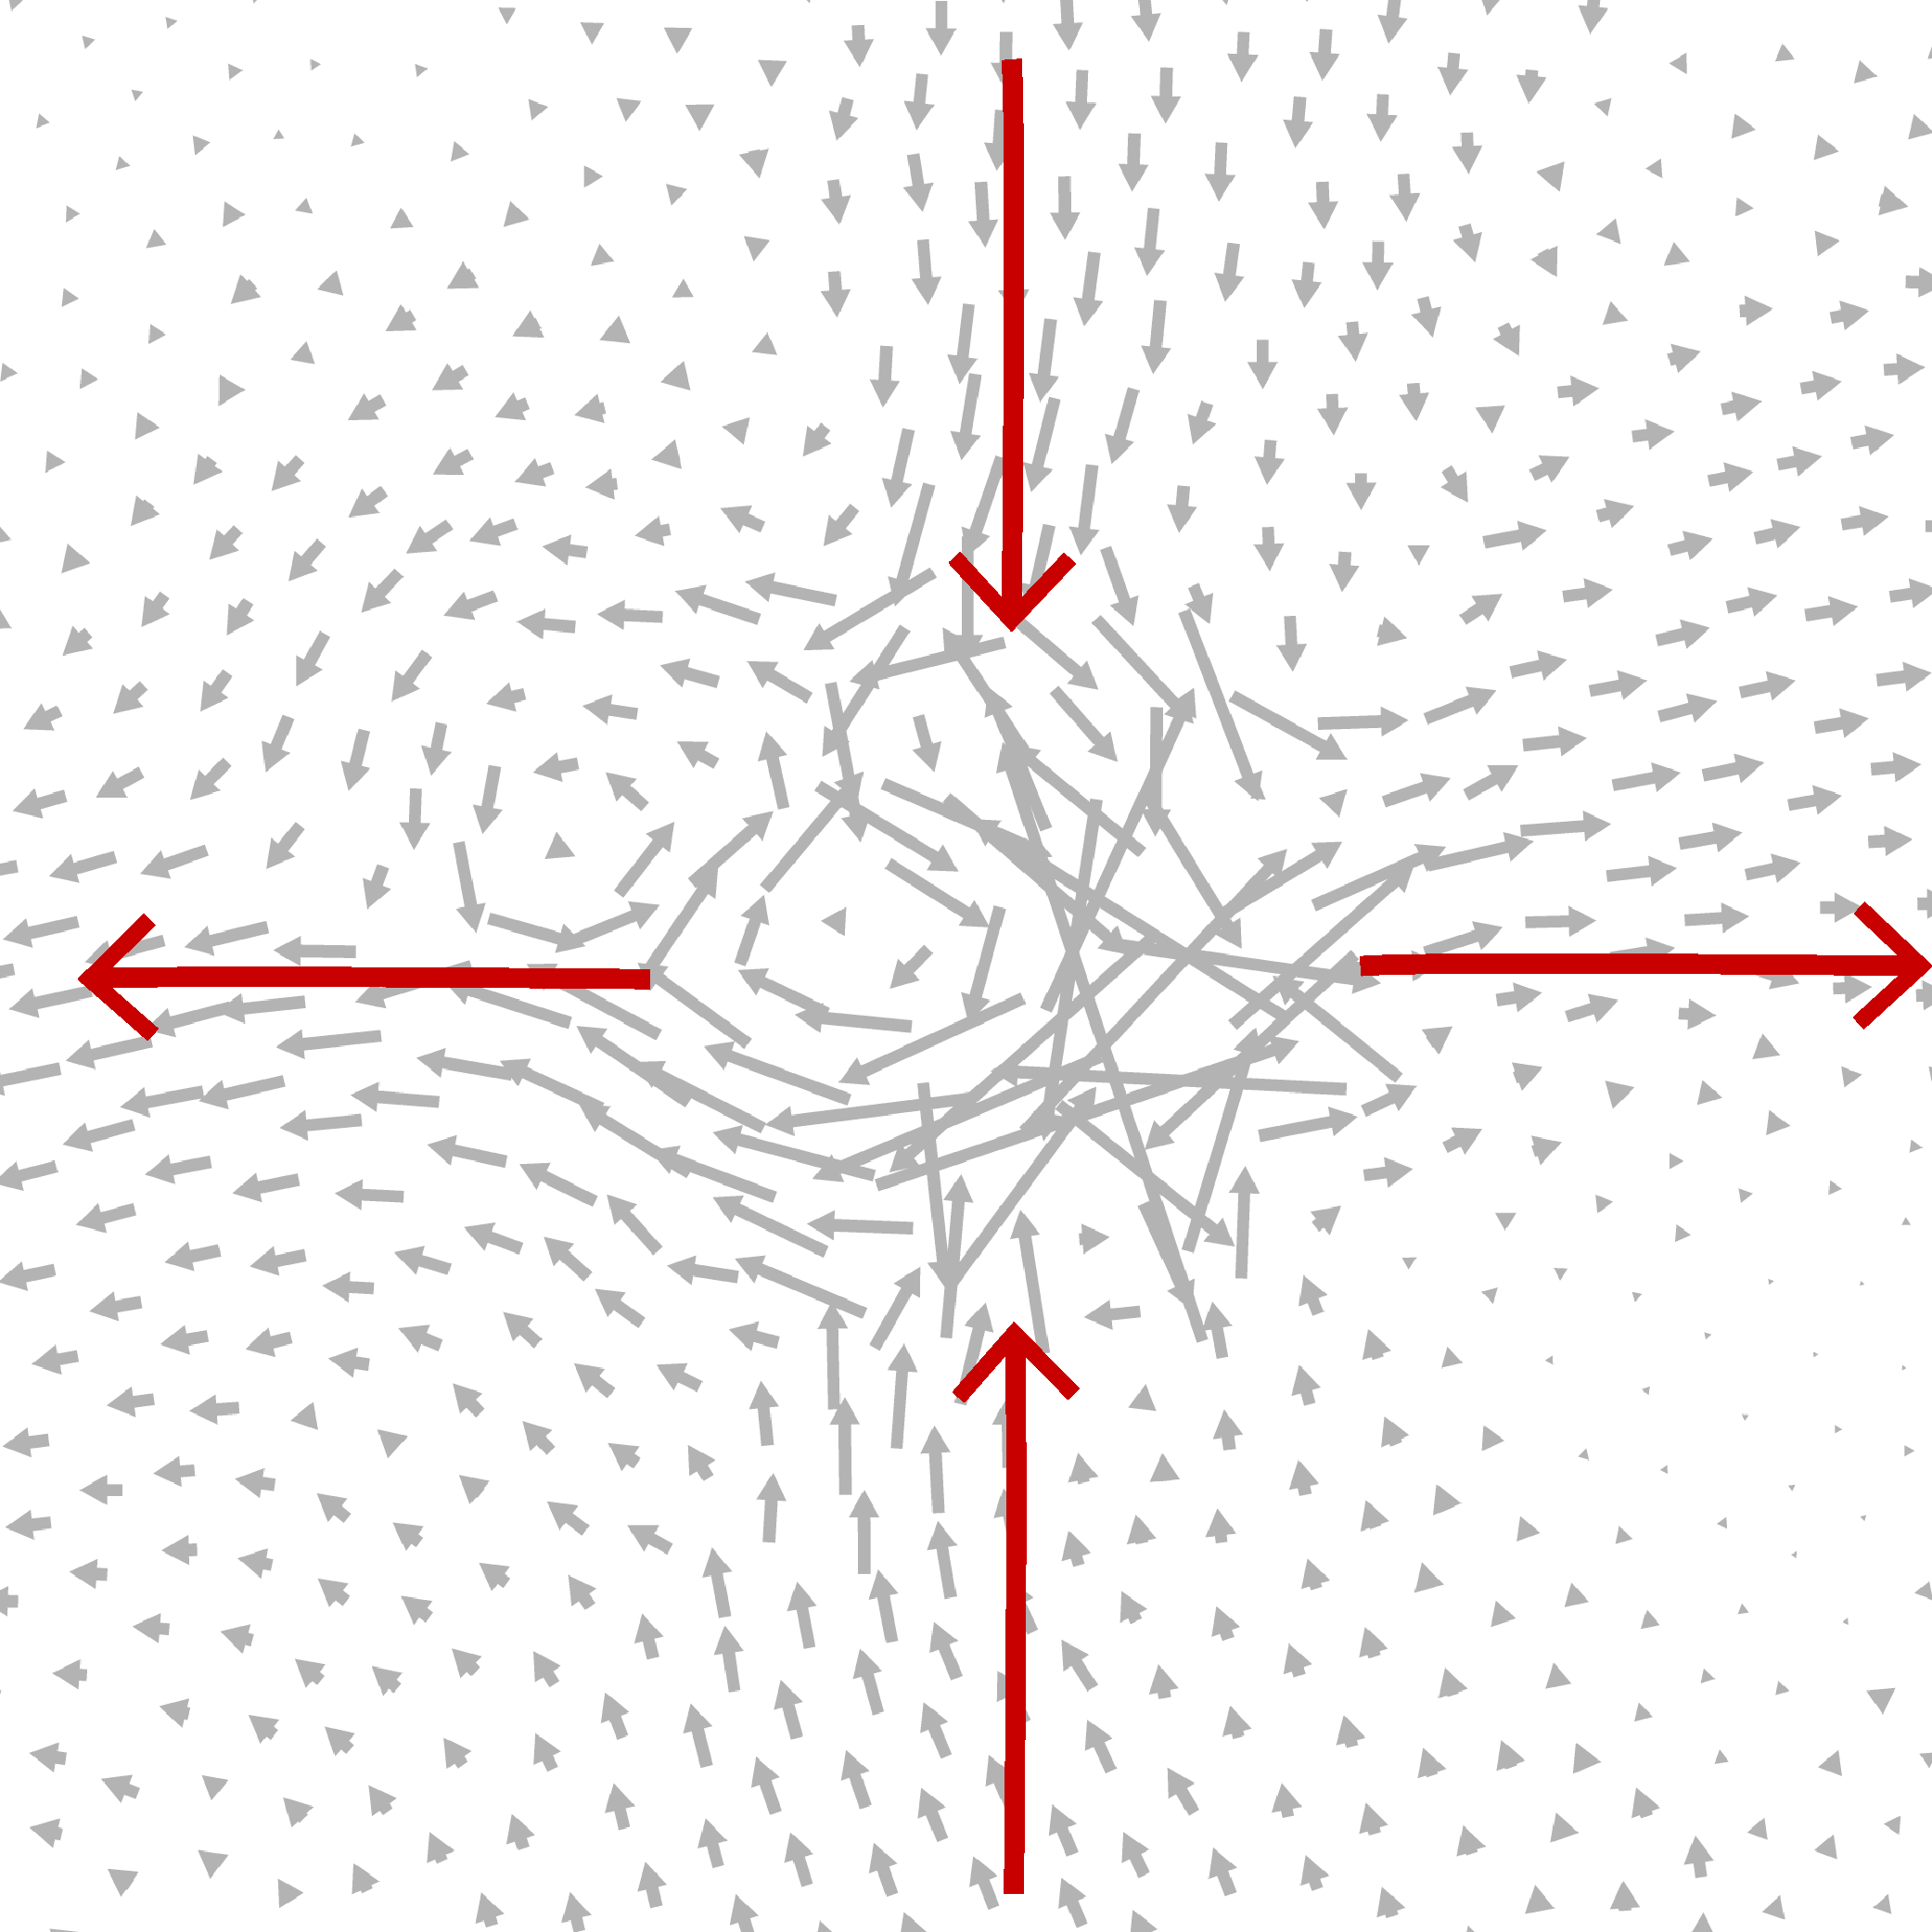
\includegraphics[width=0.85\linewidth]{1.b-exc_pureshear/zoomin-2.pdf}\caption{In another axis, there's extensile flow.}

\onslide<9>\centering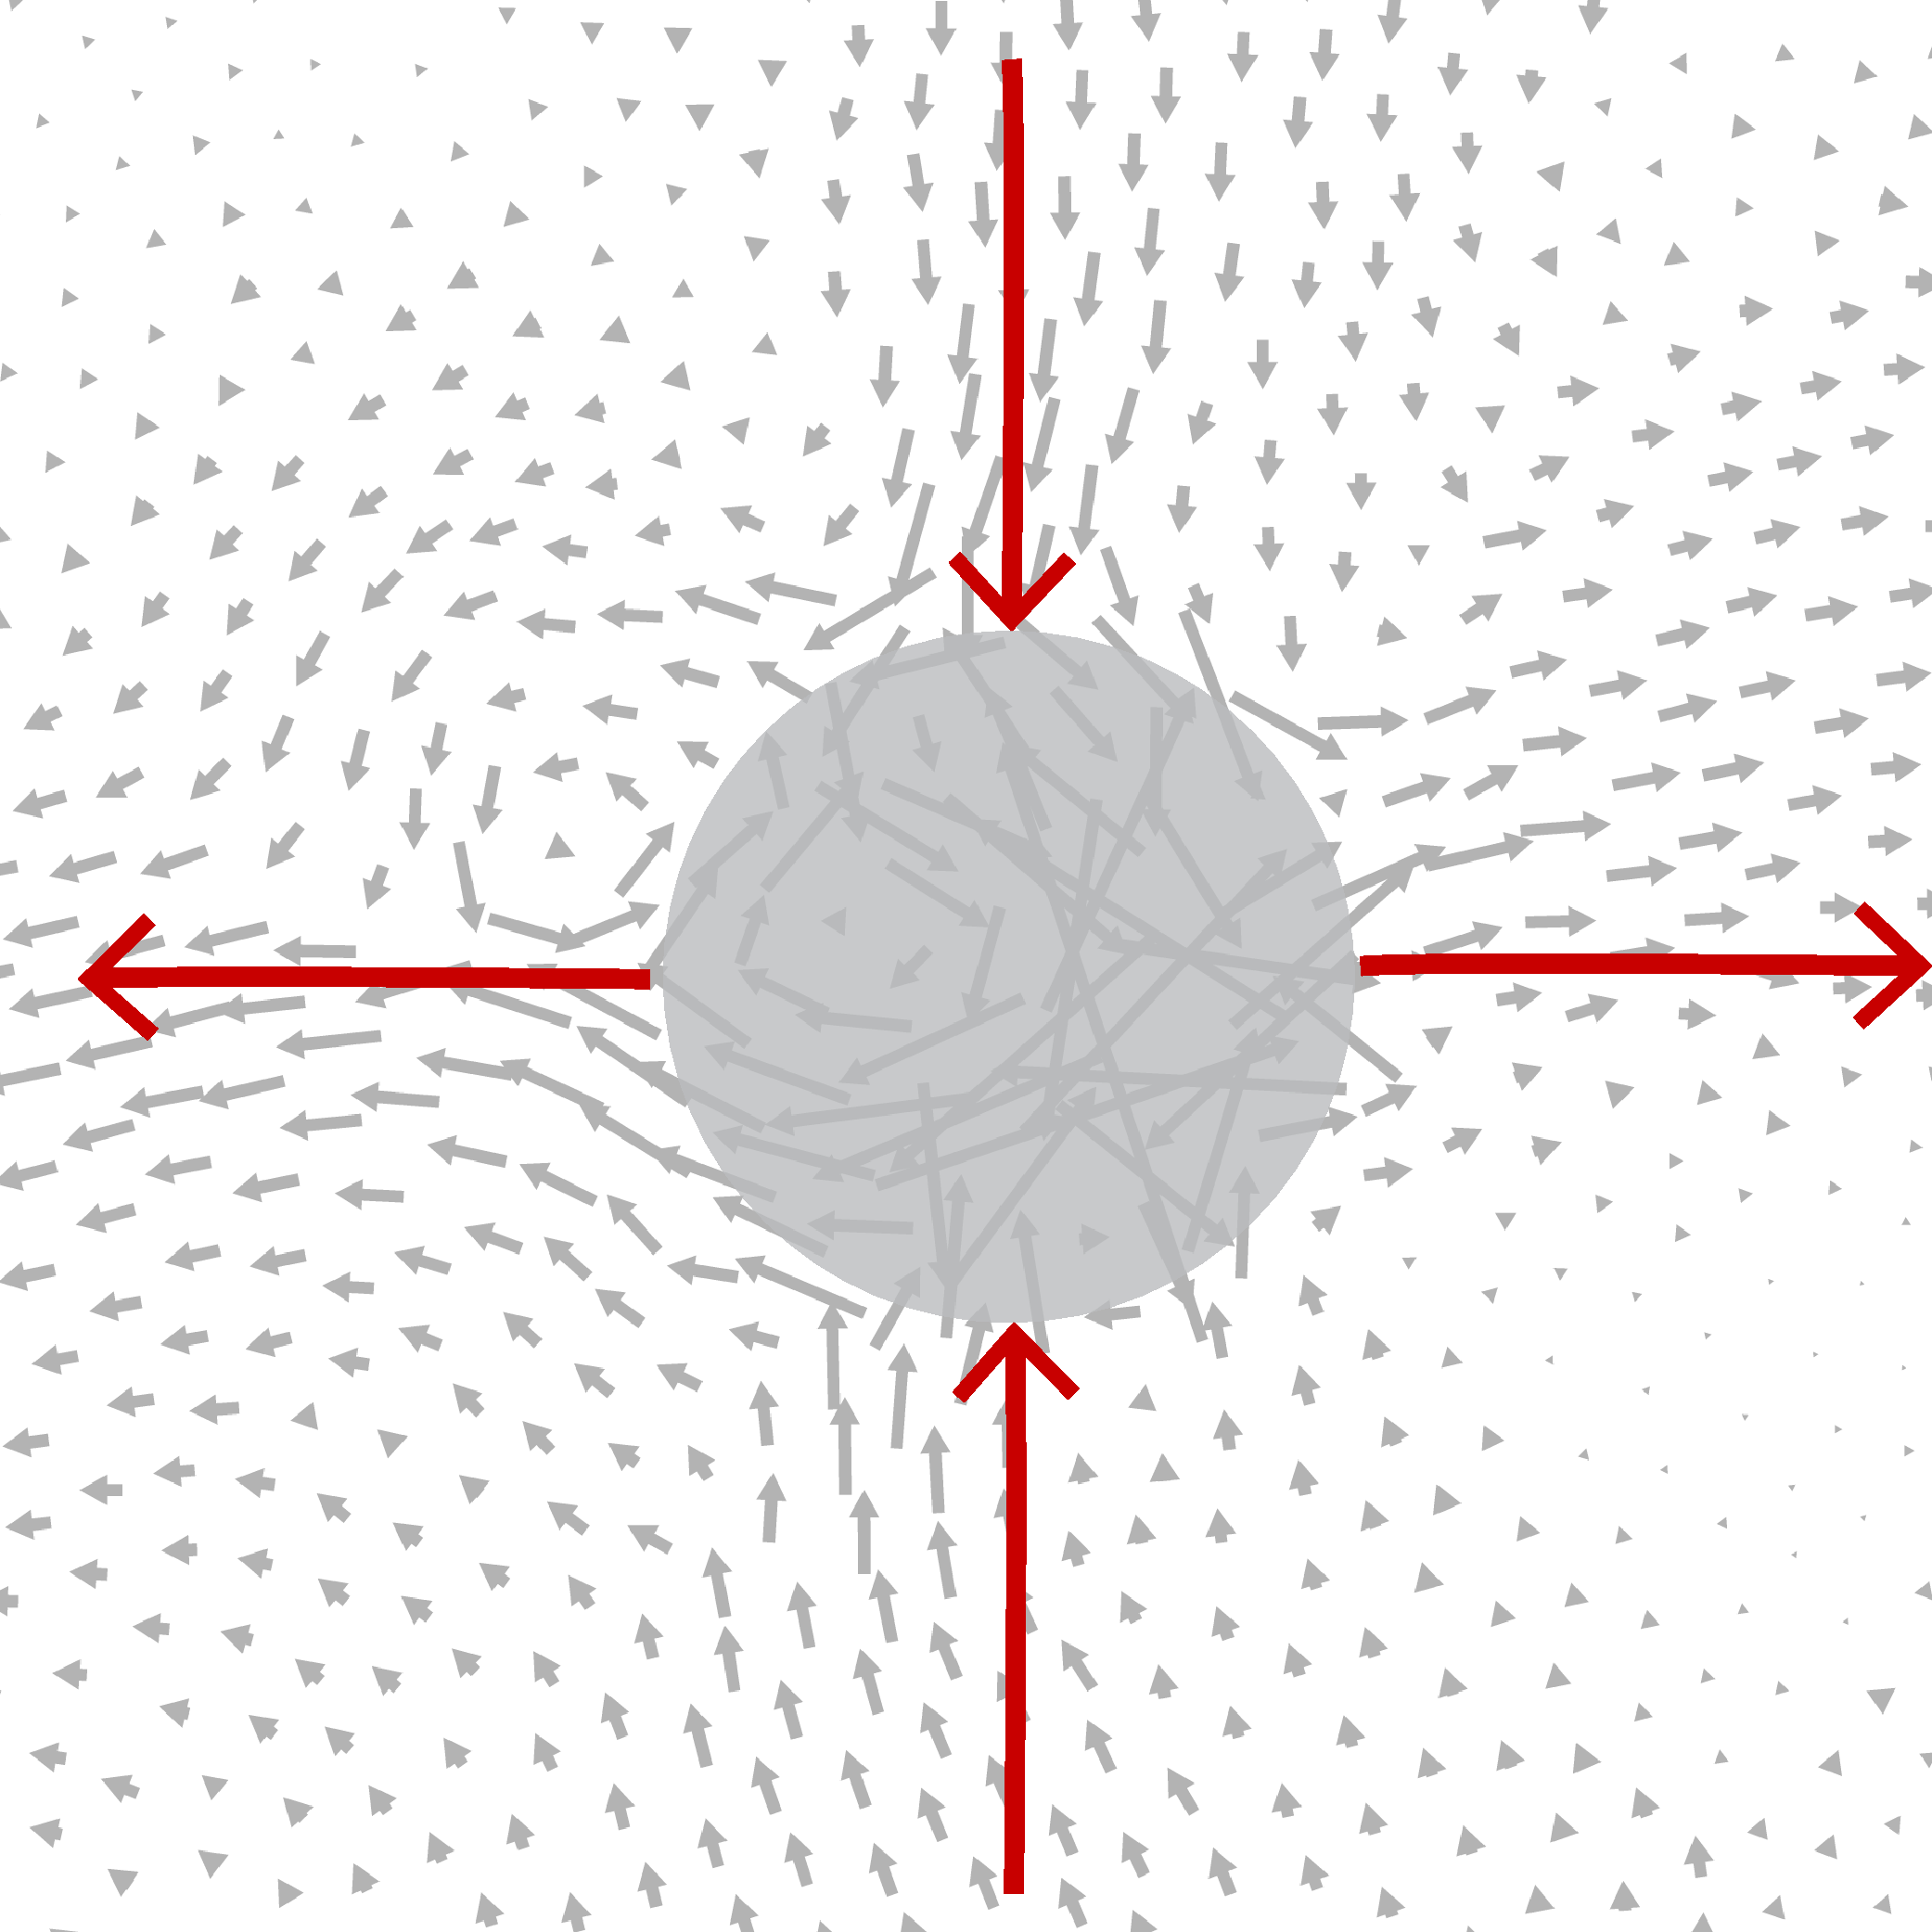
\includegraphics[width=0.85\linewidth]{1.b-exc_pureshear/zoomin-3.pdf}\caption{Compressive + extensile flow = \textbf{a pure shear deformation} {\footnotesize (Lemaitre, \textit{PRL} 2014).}}

\onslide<10>\centering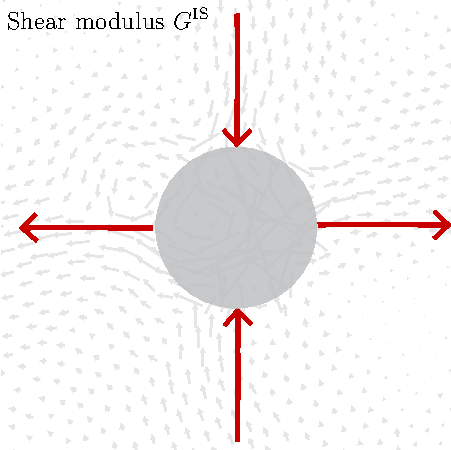
\includegraphics[width=0.85\linewidth]{1.b-exc_pureshear/zoomin-7.pdf}\caption{Compressive + extensile flow = \textbf{a pure shear deformation} {\footnotesize (Lemaitre, \textit{PRL} 2014).}}

\onslide<11>\centering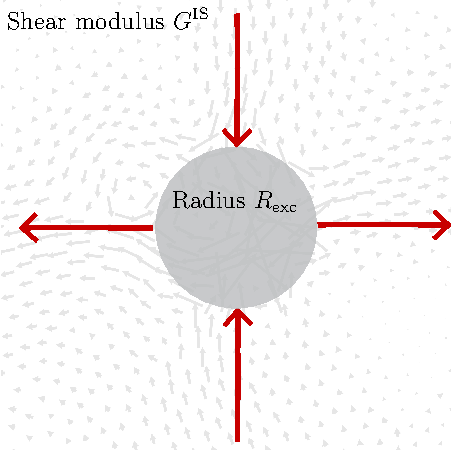
\includegraphics[width=0.85\linewidth]{1.b-exc_pureshear/zoomin-8.pdf}\caption{Compressive + extensile flow = \textbf{a pure shear deformation} {\footnotesize (Lemaitre, \textit{PRL} 2014).}}

\onslide<12-14>\centering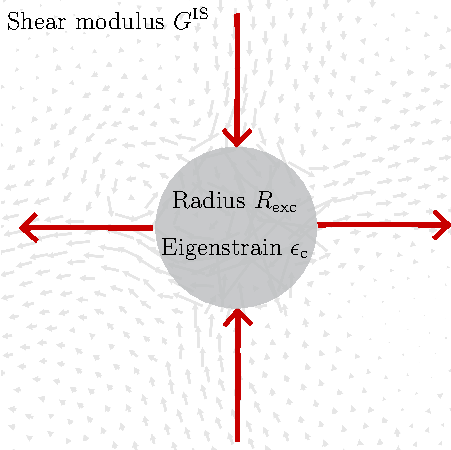
\includegraphics[width=0.85\linewidth]{1.b-exc_pureshear/zoomin-9.pdf}\caption{Compressive + extensile flow = \textbf{a pure shear deformation} (Lemaitre, \textit{PRL} 2014).}

\onslide<15->\centering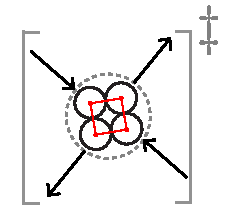
\includegraphics[width=0.85\linewidth]{1.b-exc_pureshear/T1transition.pdf}\caption{A structural motif underlie the localized pure shear, e.g., T1 transition in 2D.}

% \onslide<9>\centering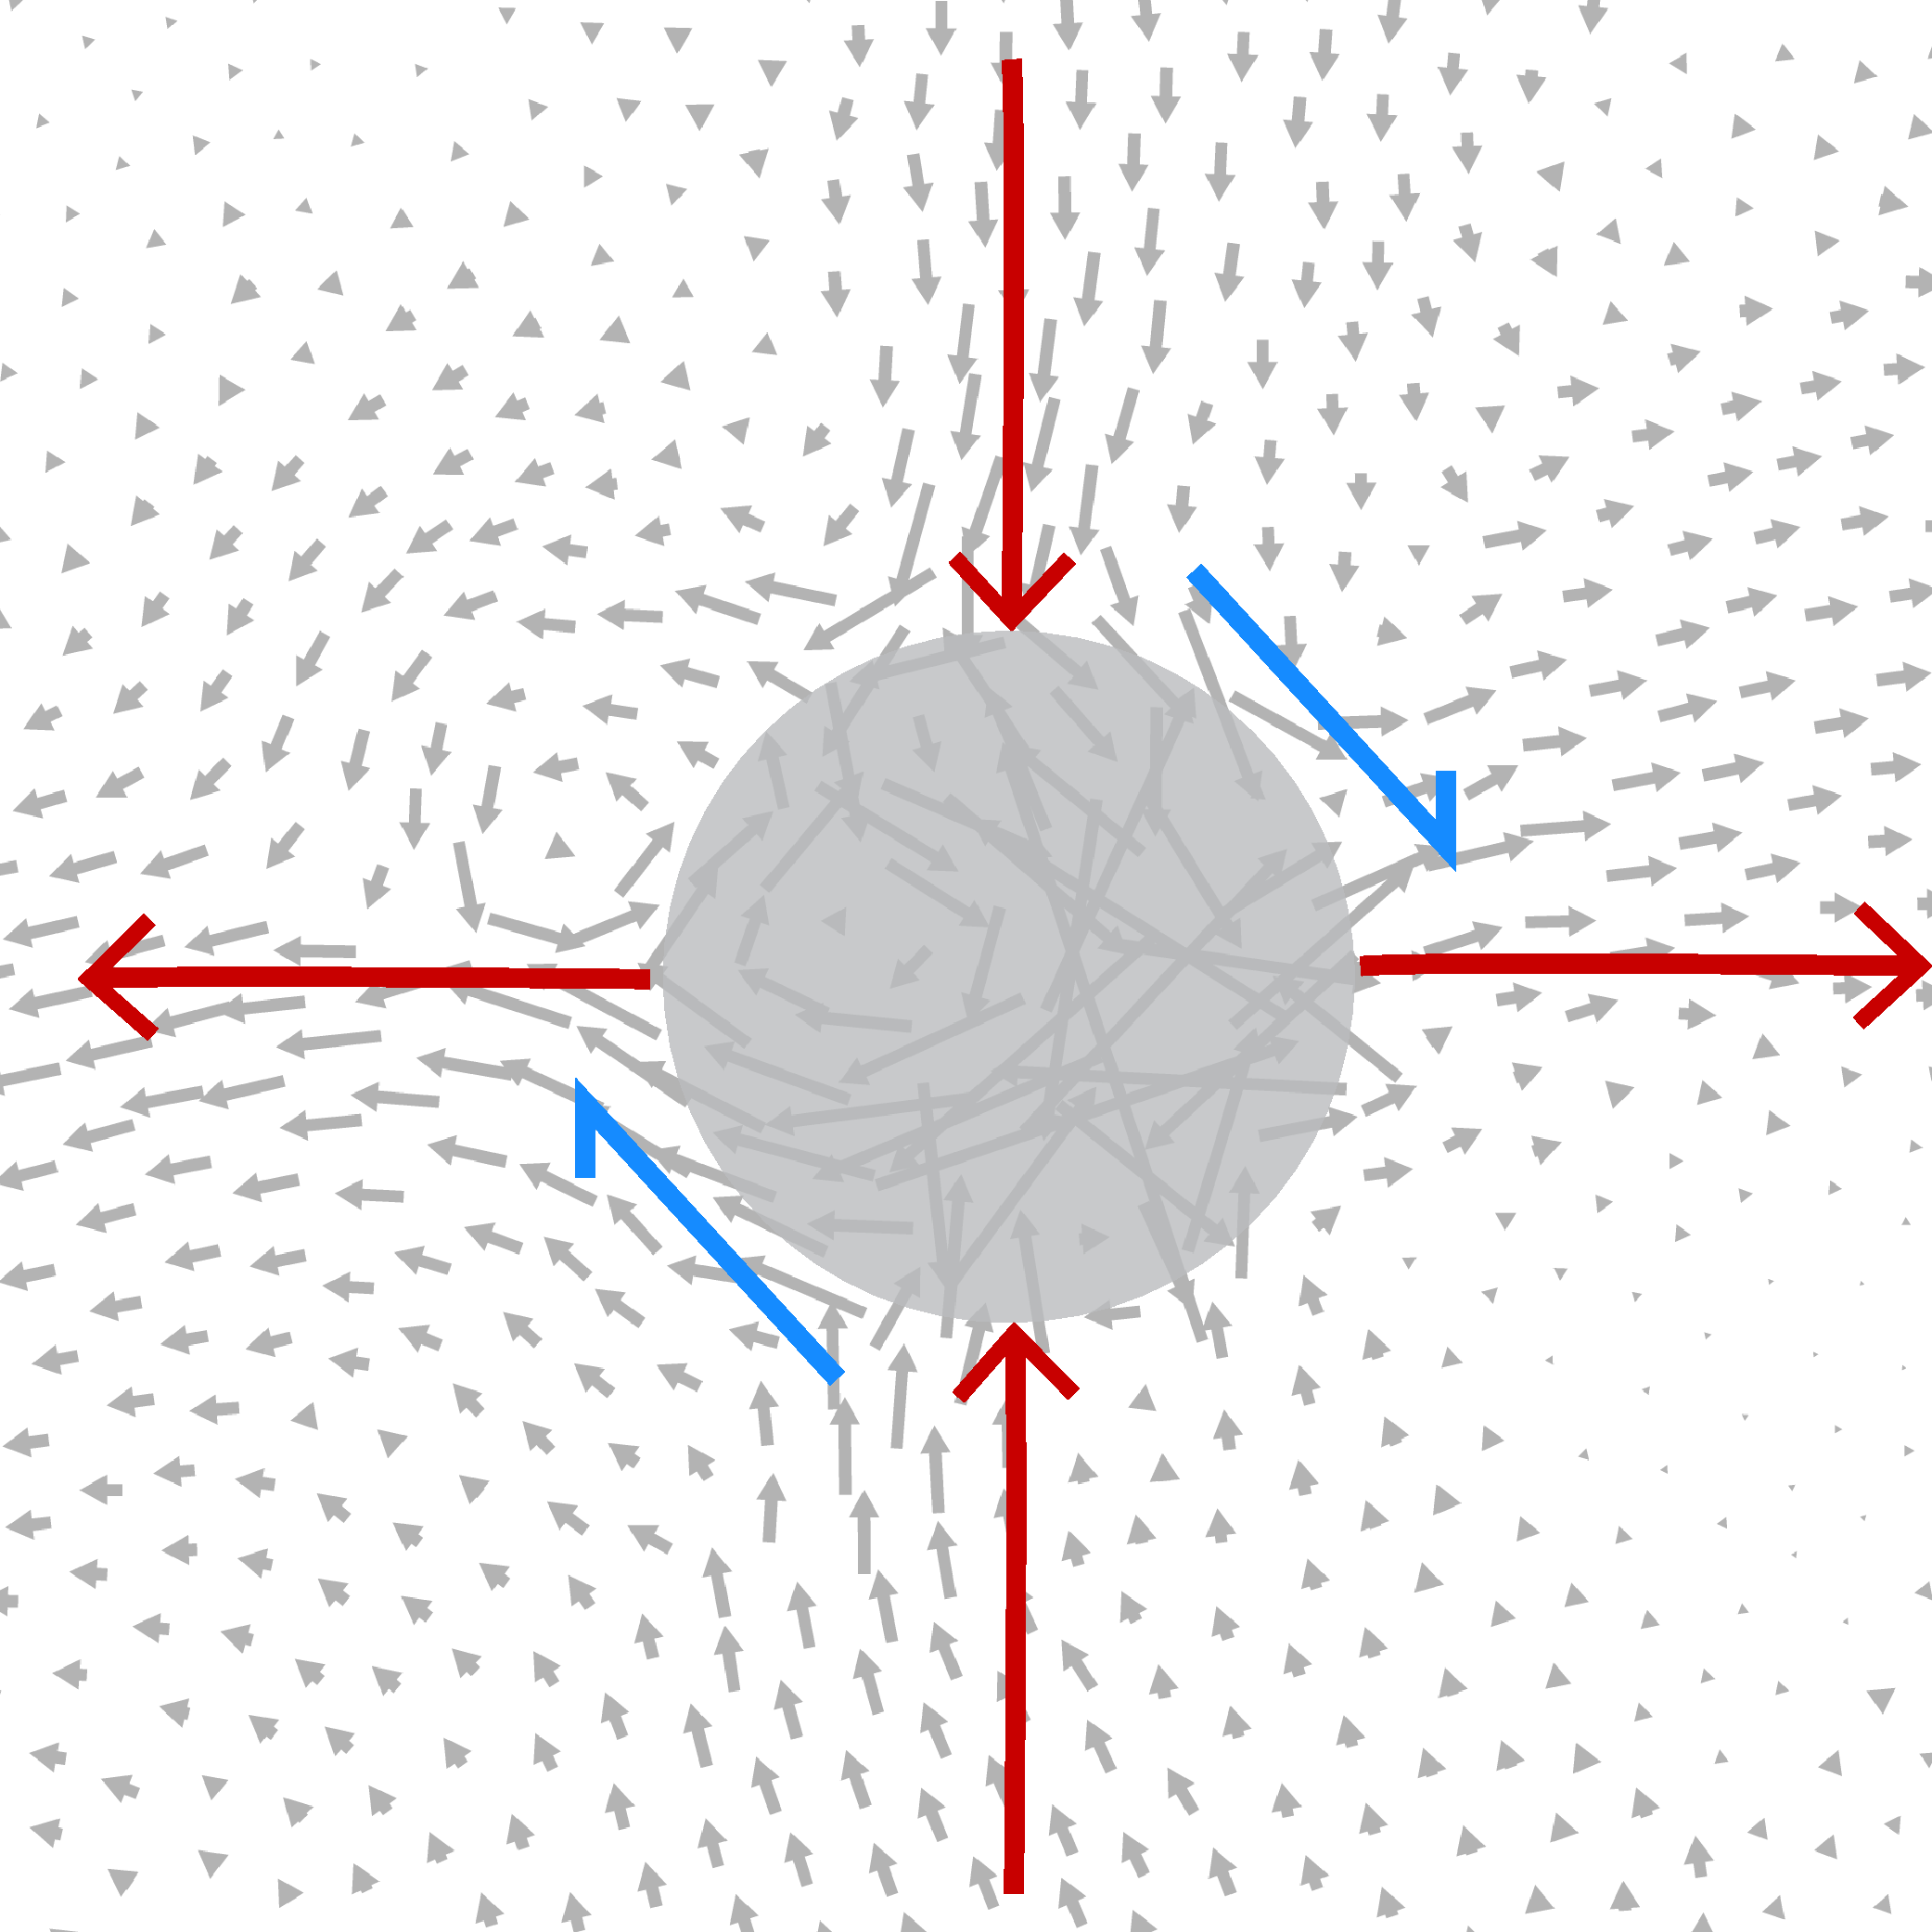
\includegraphics[width=0.85\linewidth]{1.b-exc_pureshear/zoomin-4.pdf}\caption{Alternatively, an excitation induces a simple shear in one side.}

% \onslide<10->\centering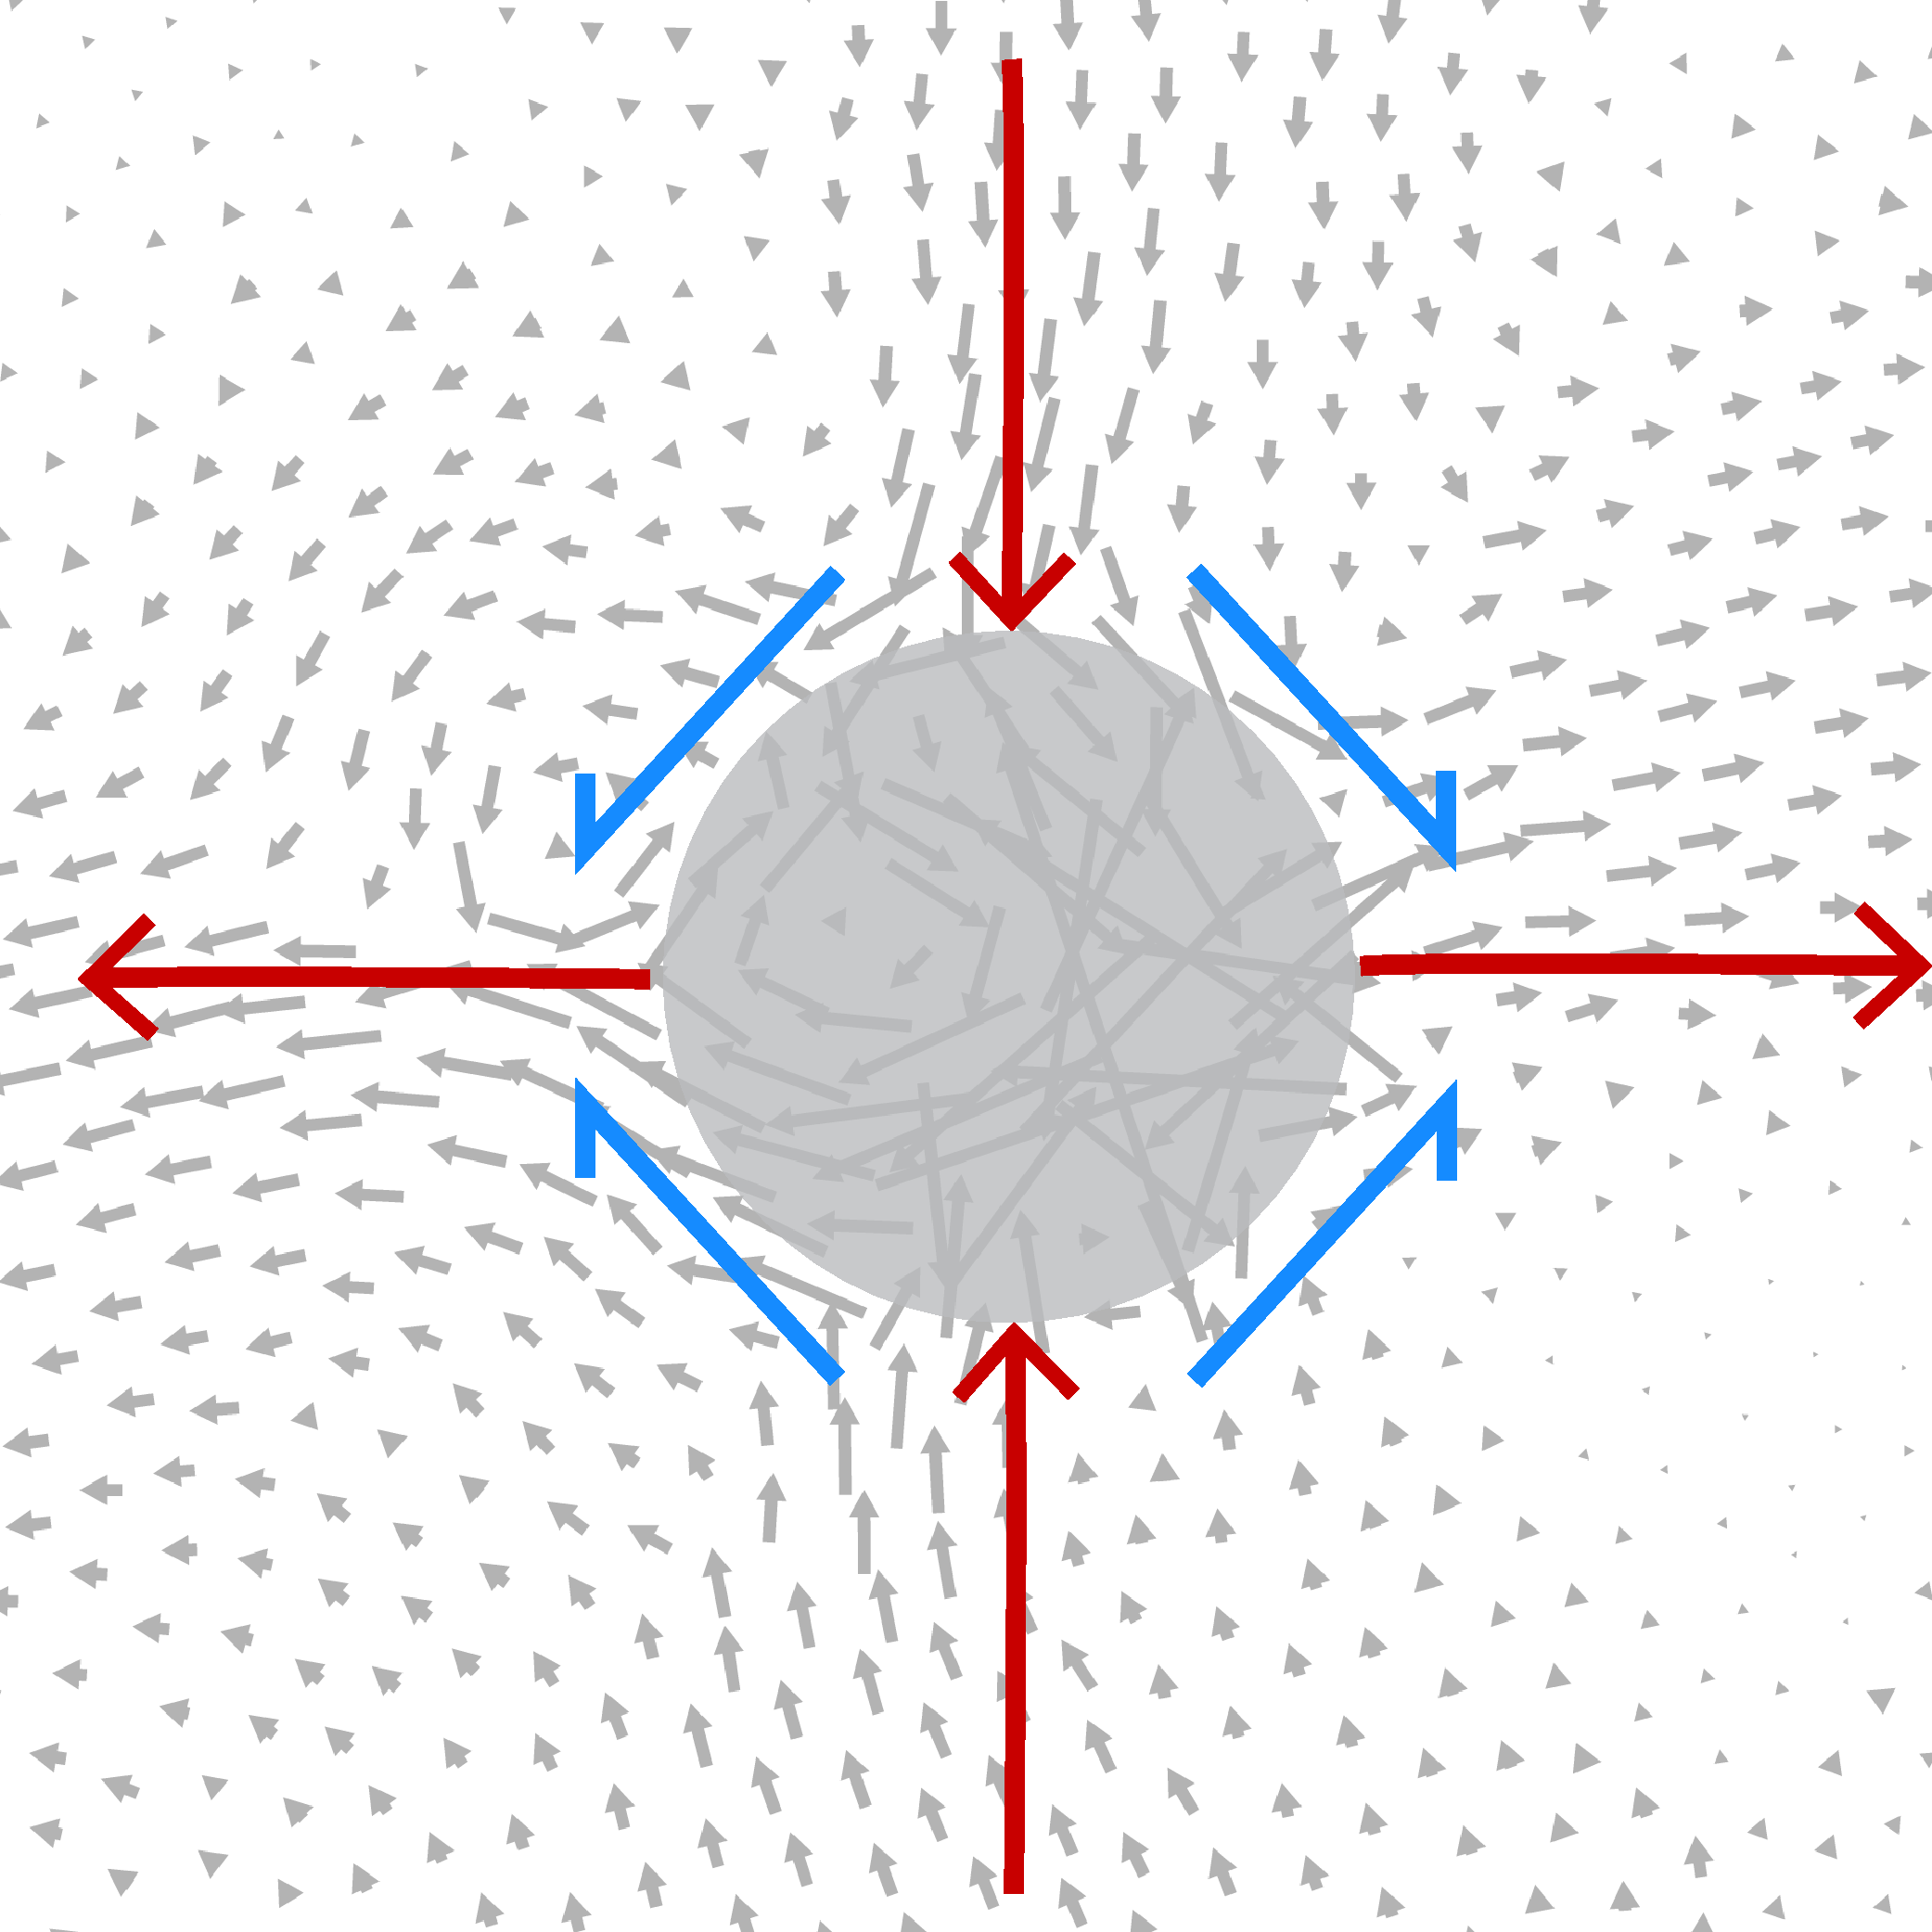
\includegraphics[width=0.85\linewidth]{1.b-exc_pureshear/zoomin-5.pdf}\caption{And induce an additional simple on the other side $\to$ \textbf{pure shear}.}
%\includegraphics[width=0.9\linewidth]{1.b-exc_pureshear/pureshear.jpg}

    
\end{overprint}
\end{figure}

\end{column}

\begin{column}[T]{0.6\textwidth}

\begin{enumerate}
\item<2-> Inherent states `=' amorphous solids %(for small deformations)

\item<13-> The linear theory of elasticity: %Energetic cost arises from the elastic reorganization of its surroundings:
\onslide<13->{
\begin{center}
\begin{minipage}{0.9\linewidth}

\begin{block}{\centering Excitation Energy Cost $J_\sigma$}

\begin{gather*}
\Delta F^\ddagger(T) = G^\mathrm{IS}(T) \left(\pi R_\mathrm{exc}^2 \right) \epsilon_c^2 \quad \text{(in 2D)}
\\
J_\sigma = \lim_{T \to 0} \Delta F^\ddagger(T)
%G^\mathrm{IS}(T) = \left\langle C_{xyxy}(\{ \* R^\alpha\})\right\rangle_\mathrm{IS}
\end{gather*}
\end{block}
\end{minipage}
\end{center}
}

\item<14-> Compute $G^\mathrm{IS}(T)$ from first-principles. (Lutsko, \textit{J. App. Phys.} (1989)).
\item<15-> Compute  $R_\mathrm{exc}$ and $\epsilon_\mathrm{c}$ from structural info, e.g., the radial distribution function. %(Hasyim, Mandadapu, \textit{J. Chem. Phys.} (2021)).
\end{enumerate}

\end{column}
\end{columns}

\end{frame}


\begin{frame}[c]\label{b.2}
\frametitle{A Theory of Localized Excitations: The Inherent-State Shear Modulus $G^\mathrm{IS}$}

\begin{columns}[c]
\begin{column}[T]{0.5\textwidth}

\begin{figure}
    \begin{overprint}
    \onslide<3-5>\centering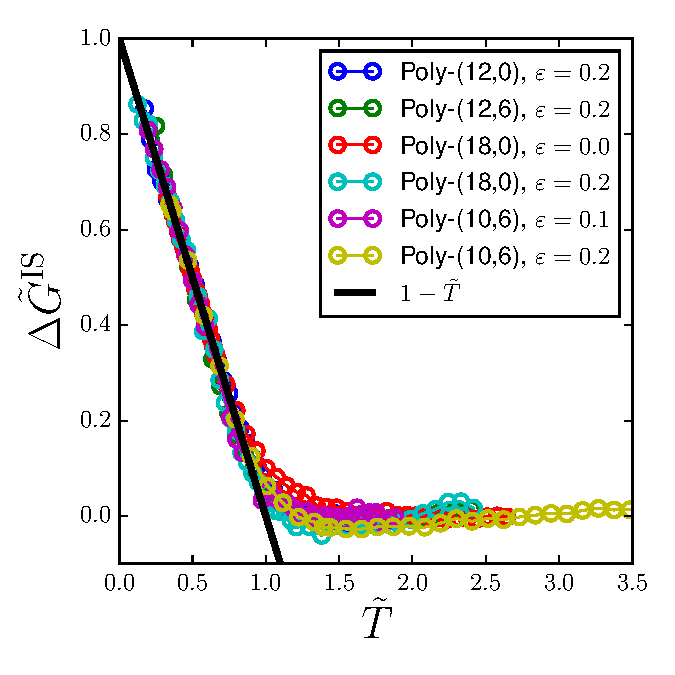
\includegraphics[width=0.85\linewidth]{b.2-exc_results_1/dimshearmodulus.pdf}\caption{Collapsed shear moduli of all poly-disperse models (Hasyim and Mandadapu,  \textit{J. Chem. Phys.} (2021)).}
    \onslide<6->\centering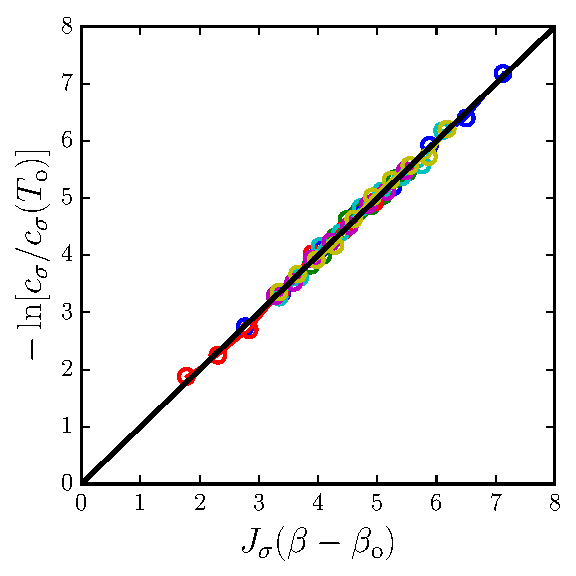
\includegraphics[width=0.85\linewidth]{b.2-exc_results_1/csigma.pdf}\caption{The observed rate $c_\sigma(T)$ of particle hopping events is also Arrhenius (Hasyim and Mandadapu,  \textit{J. Chem. Phys.} (2021); Keys, et al. \textit{Phys. Rev. X} (2011)).}
    \end{overprint}
\end{figure}

\end{column}

\begin{column}[T]{0.5\textwidth}
\begin{itemize}
    \item<2-> Linear increase as $T\to 0$ persists in all polydisperse glass formers considered.  \uncover<3->
    {    
    \begin{gather*}
    \Delta \widetilde{G}^\mathrm{IS}\left(\tilde{T}\right) := \frac{G^\mathrm{IS}(T)-G^\mathrm{IS}_\infty}{G^\mathrm{IS}(0)-G^\mathrm{IS}_\infty} ; \quad \tilde{T} := \frac{T}{T_\mathrm{p}}
    \\
    \Delta \widetilde{G}^\mathrm{IS}\left(\tilde{T}\right) = \begin{cases}
    1-\tilde{T}  & \tilde{T} \leq 1
    \\
    0 & \tilde{T} > 1
    \end{cases} \label{eq:subtractedgis}
    \end{gather*}
    }
    \item<4-> Existence of cross-over temperature $T_\mathrm{p} < T_\mathrm{o}$ delineating low-$T$ linear regime from the high-$T$ plateau. 
    \uncover<5->
    {
    \begin{block}{\centering Linearity of $G^\mathrm{IS}$}
    Since $\Delta F^\ddagger(T) \sim G^\mathrm{IS}(T)$, the rate of excitation events $k_\mathrm{exc}(T) \sim e^{-\beta J_\sigma} $ is effectively Arrhenius!
    \end{block}
    }
\end{itemize}
\end{column}

\end{columns}
    
\end{frame} 
\begin{frame}[c]\label{b.3}
\frametitle{A Theory of Localized Excitations: Numerical Results} % $J_\sigma$

\begin{columns}

\begin{column}{0.6\linewidth}

\onslide<2->\begin{table}[h]
\begin{tabular}{lccccc}
\hline\hline
Glass Former  & Measured$^\ddagger$ $J_\sigma$  & Predicted$^\dagger$ $J_\sigma$  \\ \hline
Poly-(12,0), ($\varepsilon=0.2$)  & \tikzmark{start1} 1.710(2)  & 1.77(2) \tikzmark{end2}  \\
Poly-(12,6), ($\varepsilon=0.2$)    & 0.914(2)  & 0.80(2)   \\
Poly-(18,0), ($\varepsilon=0.0$)    &  6.69(1)  & 10.2(6)   \\
Poly-(18,0), ($\varepsilon=0.2$)    & 2.034(3)  & 2.18(1)   \\
Poly-(10,6), ($\varepsilon=0.1$)    & 1.365(2)  & 1.56(3)  \\
Poly-(10,6), ($\varepsilon=0.2$)    & 0.700(2)  & 0.588(2)   \\
\hline\hline
\only<3->{\begin{tikzpicture}[overlay,remember picture]
  \draw[red, thick] ([shift={(-1ex,1.75ex)}]pic cs:start1) rectangle ([shift={(1ex,-0.75ex)}]pic cs:end2);
\end{tikzpicture}
}
\end{tabular}
\vspace{-12pt}
\caption{\footnotesize $^\ddagger$ Obtained from the rate of particle hopping events in MD simulations.$^\dagger$ Using the final formula, with shear modulus $G^\mathrm{IS}$ and RDF $g(\tilde{r})$ as input. (Hasyim and Mandadapu, \textit{J. Chem. Phys.}, 2021)} \label{tab:summary}
\end{table}
\vspace{-12pt}
\begin{itemize}
    \item<3-> Without fitting to relaxation data, predicted activation energy is in reasonable agreement with MD simulations!
    \item<5-> Strain profile also matches qualitatively with those observed in literature.
\end{itemize}
\end{column}

\begin{column}{0.4\linewidth}

\begin{figure}
    \centering
    \begin{overprint}
    \onslide<4>\centering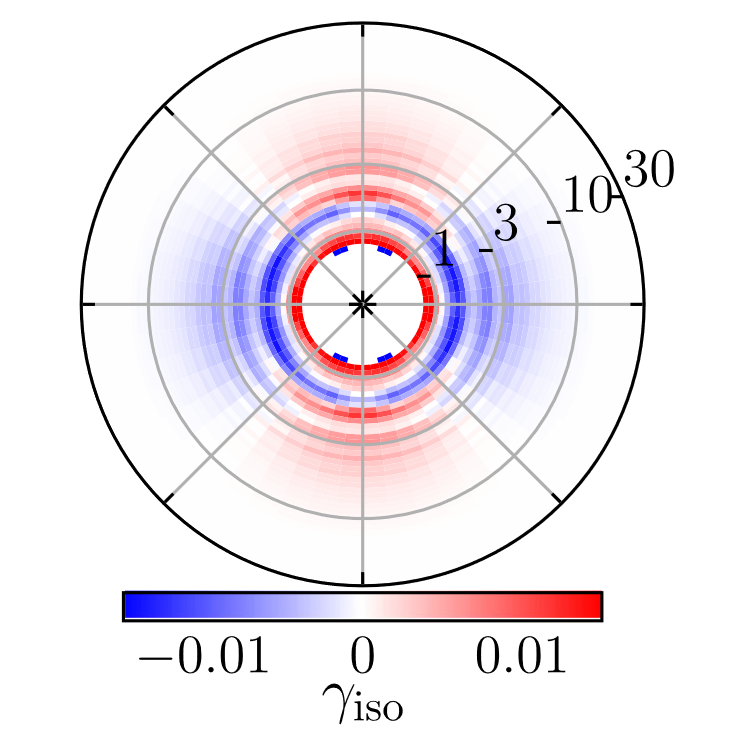
\includegraphics[width=0.95\linewidth]{b.3-exc_results_2/giso_lit.png}\caption{Strain profile from MD simulations (Chacko, et. al. \textit{Phys. Rev. Lett.} 2021)}
    \onslide<5->\centering\includegraphics[width=\linewidth]{b.3-exc_results_2/giso-2.pdf}\caption{From linear theory of elasticity}
    \end{overprint}
    \label{fig:my_label}
\end{figure}

\end{column}

\end{columns}

\end{frame} 

\begin{frame}
\vspace{20pt}
\section{A Theory of Onset Temperature in 2D}

\centering\fbox{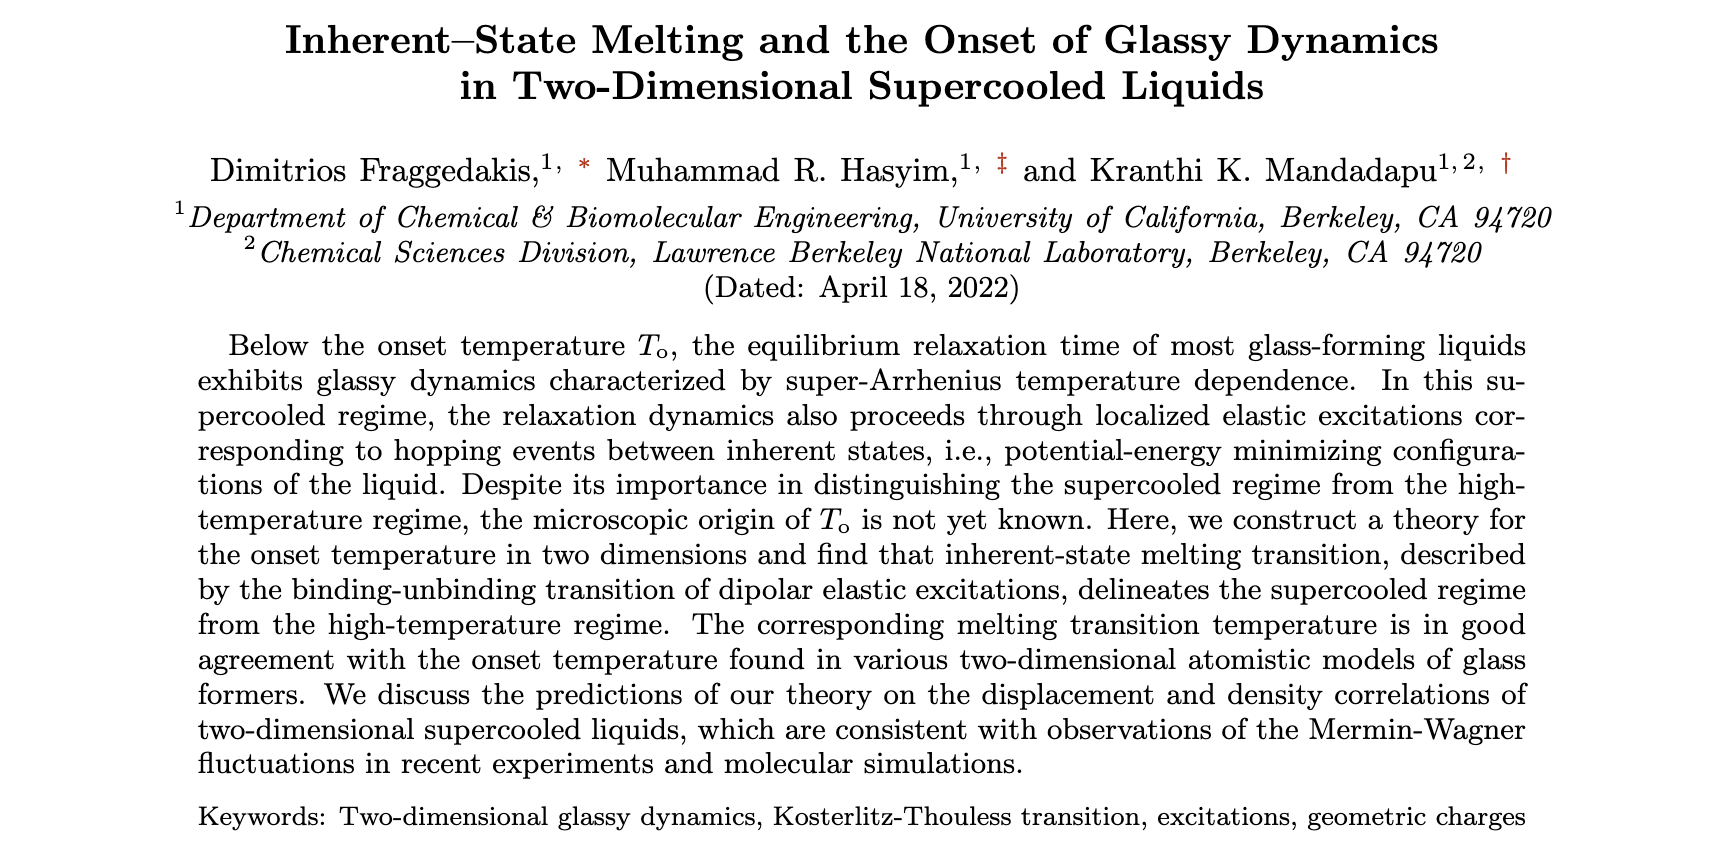
\includegraphics[height=0.5\textheight]{ismeltingpaper_screen.png}}%{section_1_image.png}

D. Fraggedakis, M.R. Hasyim, K.K. Mandadapu, \textit{PNAS} 120 (14) e2209144120 (2023)

\end{frame}

% Part C: 2D Onset Temperature Theory

\begin{frame}[c]\label{c.1}
\frametitle{A Theory of Onset Temperature in 2D: The Mean-Squared Displacement}


\begin{columns}[T]
\begin{column}[T]{0.4\textwidth}
\vspace{-12pt}
\begin{figure}[t]
%\includegraphics[height=0.65\textheight]{figures/pel_hopping.png}
\begin{overprint}

\onslide<3>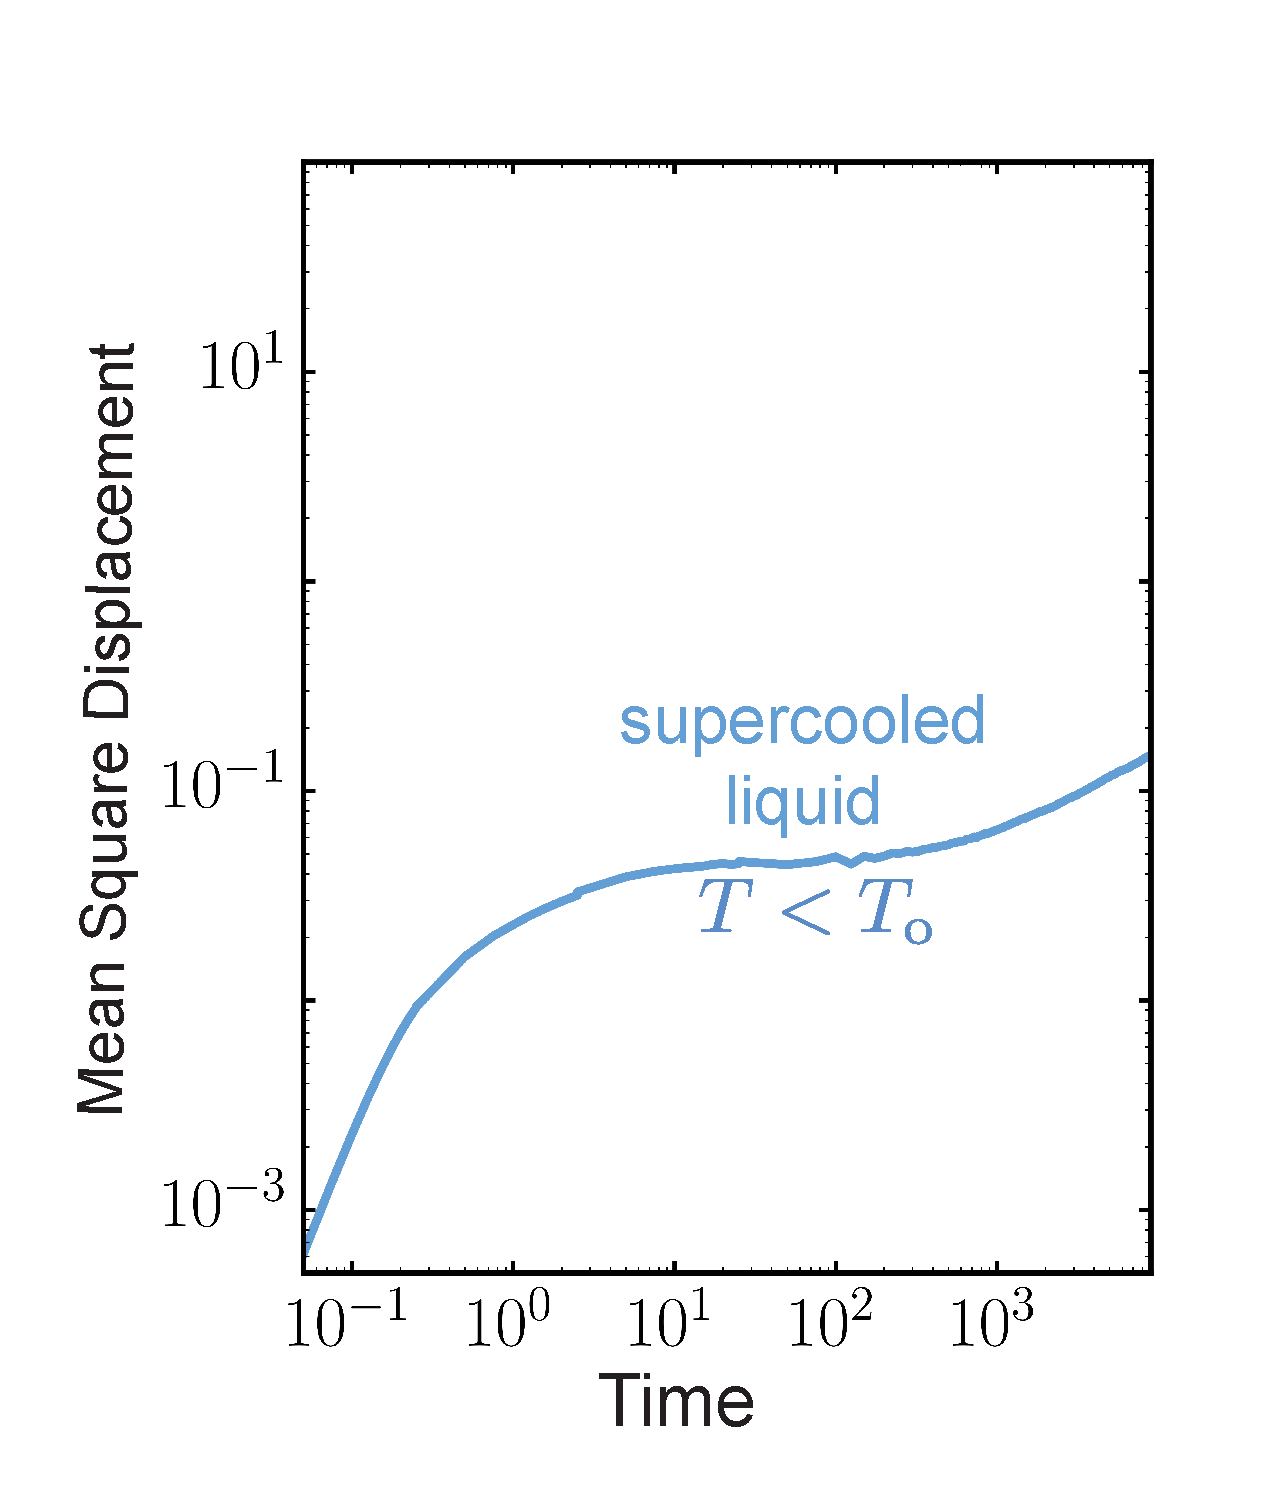
\includegraphics[height=0.75\textheight]{c.1-kt_msdintro/msd-supercooledliq-0.pdf}\caption{The MSD of a polydisperse system at $ T \approx 0.50 T_\mathrm{o}$}


\onslide<4-5>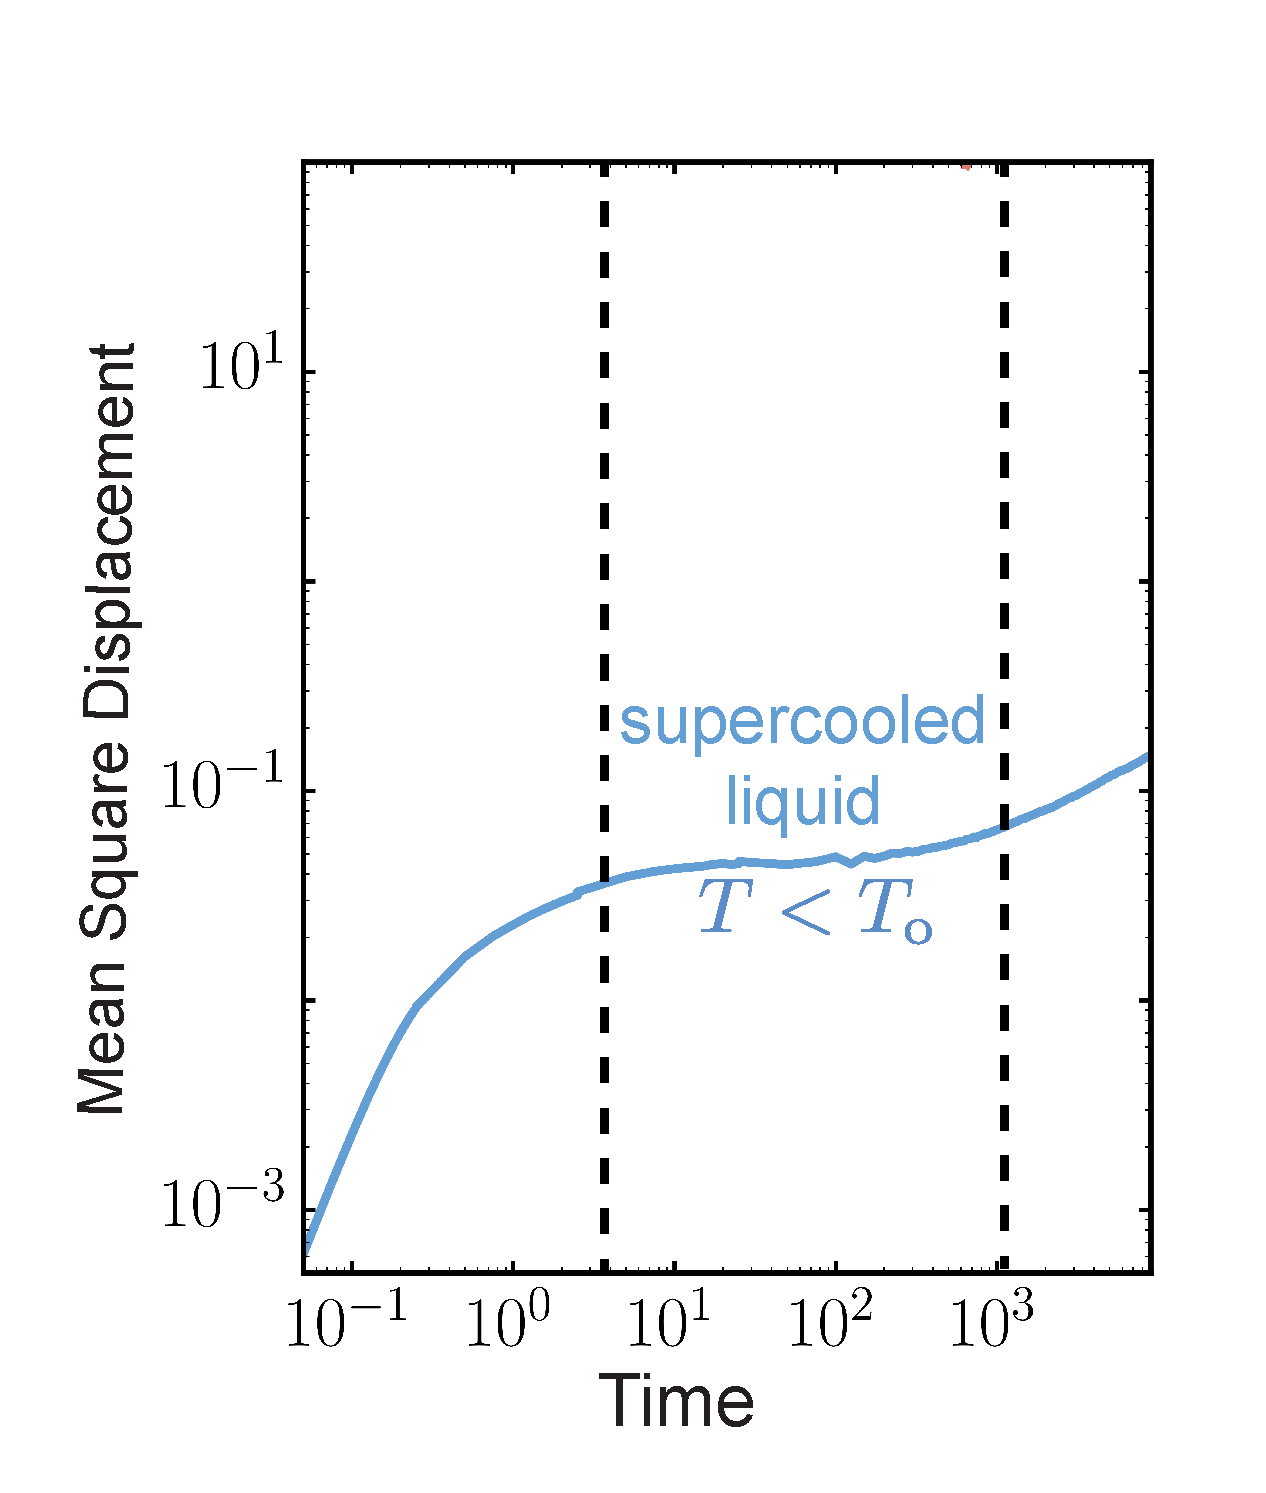
\includegraphics[height=0.75\textheight]{c.1-kt_msdintro/msd-supercooledliq-1.pdf}\caption{The MSD of a polydisperse system at $ T \approx 0.50 T_\mathrm{o}$}

\onslide<6>\includegraphics[height=0.75\textheight]{c.1-kt_msdintro/msd-supercooledliq-2.pdf}\caption{The MSD of a polydisperse system at $ T \approx 0.50 T_\mathrm{o}$ with snapshot of excitation events (in yellow)}


%\onslide<7>\includegraphics[height=0.75\textheight]{c.1-kt_msdintro/msd-supercooledliq-3.pdf}\caption{The MSD of a supercooled liquid $ T \approx 0.50 T_\mathrm{o}$ with snapshot of excitation events (in yellow)}


\onslide<7>\includegraphics[height=0.75\textheight]{c.1-kt_msdintro/msd-supercooledliq-4.pdf}\caption{The MSD at high temperatures $T \approx 2.0 T_\mathrm{o}$}


\onslide<8->\includegraphics[height=0.75\textheight]{c.1-kt_msdintro/msd-supercooledliq-5.pdf}\caption{The MSD at high temperatures $T \approx 2.0 T_\mathrm{o}$ with snapshots of mobile regions (in yellow)}


\end{overprint}
\end{figure}


\end{column}

\begin{column}[T]{0.6\textwidth}



\only<2->{Observe the mean-squared displacement (MSD) of a particle}
\begin{enumerate}
\item<4-> $T < T_\mathrm{o}$: ``Plateau" region\uncover<5->{, shearing yields \textbf{solid} behavior}\uncover<6->{, filled with \textbf{rare excitation events}} %$t \sim \langle \tau_\mathrm{jump} \rangle \ll \langle \tau_\mathrm{eq} \rangle$)
\item<7-> $T > T_\mathrm{o}$: Immediate diffusion, shearing yields \textbf{fluid} behavior\uncover<8->{, populated with \textbf{many mobile regions}.} 
\end{enumerate}

\onslide<9->{\begin{block}{\centering \large Origin of Onset Temperature}
\onslide<10->{\centering Onset of glassy dynamics is linked to a "melting" transition at intermediate timescales $t \ll \tau_\mathrm{eq}$}


\onslide<11->{\centering An elastic solid $ \leftrightarrow $ a fluid

%At intermediate timescales ($t \sim \langle \tau_\mathrm{jump} \rangle \ll \langle \tau_\mathrm{eq} \rangle$)
}
\end{block}

}

\vspace{10pt}

\km{\onslide<12->{\centering \Large What is the mechanism for the "melting" transition?}}

\end{column}
\end{columns}



\end{frame}


% \begin{frame}{A Theory of Onset Temperature in 2D: The Role of Entropy}

% \begin{figure}
%     \centering
%     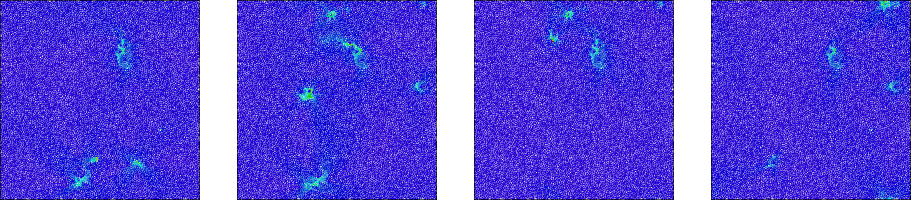
\includegraphics[height=0.375\textheight]{3.d-kt_geomcharges/excs.png}
%     \caption{Mobile regions at $T \approx 0.53 T_\mathrm{o}$ and $t \ll \tau_\mathrm{eq}$, sampled from trajectories starting from the same initial configuration $\{\* R_0^\alpha\}$ $\to$ \textbf{isoconfigurational ensemble} (Widmer-Cooper, Harrowell, Fynewever, \textit{PRL}, 2004).} %
% \end{figure}
% % \begin{columns}
% % \begin{column}{0.5\linewidth}
% % \begin{itemize}
% %     \item T
% % \end{itemize}
% % \end{column}

% % \begin{column}{0.5\linewidth}
% %hint for onset temperature $T_\mathrm{o}$ lies in the mathematical model for the localized pure-shear excitation
% \vspace{-14pt}
% \begin{itemize}
% \item<2-> The free-energy of formation for a localized pure-shear excitation
% \begin{equation*}
% \onslide<3->{\Delta F_\mathrm{f} = \underbrace{E_\mathrm{c}}_{\substack{\text{Strain elastic} \\ \text{energetic cost}}}} \onslide<4->{-\underbrace{2 k_\mathrm{B} T \ln \left(\sqrt{2 \pi} \frac{R}{R_\mathrm{exc}} \right)}_{\substack{\text{Entropy gain} \\ \text{(translation + orientation)}}}} \onslide<5->{< 0} 
% \end{equation*}
% \onslide<5->{In the thermodynamic limit ($R \to \infty$), excitations are always favored (\textit{no transition})!} 
% %\item<7-> \textbf{Analogy to electrostatics: geometric dipole} with dipole-moment vector $\mathbf{d}$, where {\large $|\* d| \sim \epsilon_\mathrm{c}$} 
% \end{itemize}
% % \end{column}
% % \end{columns}

% % \begin{figure}
% % \vspace{-9pt}
% % \begin{overprint}

% % \onslide<2-7>\centering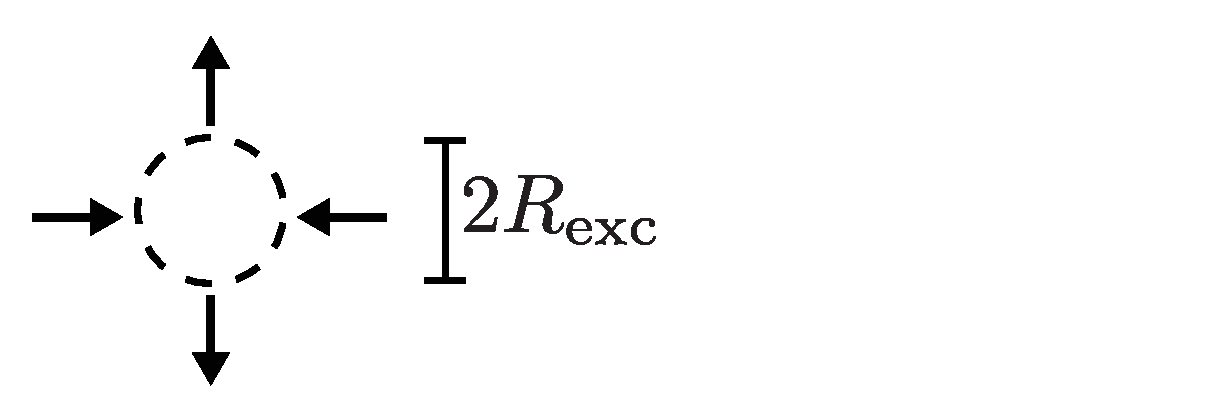
\includegraphics[width=0.75\linewidth]{3.d-kt_geomcharges/chargesequiv-0.pdf}%\caption{Testing}

% % \onslide<8>\centering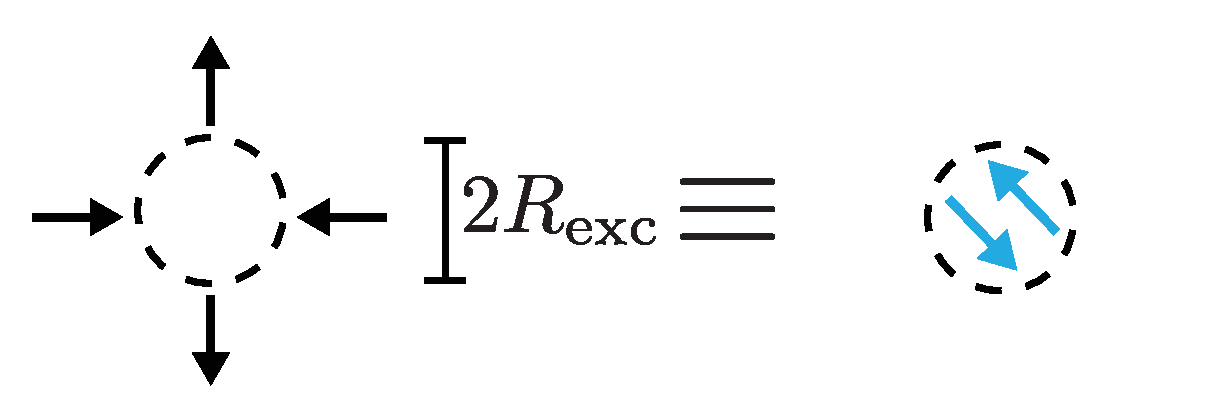
\includegraphics[width=0.75\linewidth]{3.d-kt_geomcharges/chargesequiv-1.pdf}%\caption{Testing}

% % %\onslide<8->\centering\includegraphics[width=0.75\linewidth]{3.d-kt_geomcharges/chargesequiv-2.pdf}


% % \end{overprint}
    
% % \end{figure}
    
% \end{frame}


\begin{frame}{A Theory of Onset Temperature in 2D: Geometric Charges \& Energy-Entropy Framework}

\begin{columns}[T]
\begin{column}[T]{0.5\textwidth}

\begin{block}{\centering \large Geometric Charges}
Mathematical analogy (unique to 2D) between elastic excitations and electrostatic multipoles
\end{block}

\begin{figure}
\centering\includegraphics[width=0.9\linewidth]{c.2-kt_geomcharges_1/chargesequiv-2.pdf}
\vspace{-5pt}
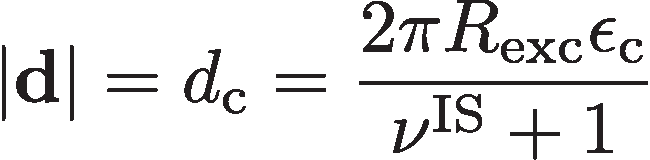
\includegraphics[width=0.6\linewidth]{c.2-kt_geomcharges_1/dipolemag.pdf}
\caption{Pure-shear excitation as bound state of \textbf{geometric dipoles}}
\end{figure}

\end{column}

\begin{column}[T]{0.5\textwidth}

\begin{block}{\centering \large Energy-Entropy Framework}
Free energy of formation for localized excitations
\end{block}

\vspace{0.3em}

\begin{equation*}
\underbrace{\Delta F_\mathrm{f}}_{\substack{\text{Free energy of} \\ \text{formation}}} = \underbrace{ \frac{d_{\mathrm{c}}^{2} Y^{\mathrm{IS}}}{8 \pi} \ln \left(\frac{R}{R_{\mathrm{exc}}}\right) }_{\substack{\text{Elastic energy cost}}} - \underbrace{2 k_\mathrm{B} T \ln \left(\sqrt{2 \pi} \frac{R}{R_\mathrm{exc}} \right)}_{\substack{\text{Entropy gain}}}
\end{equation*}

\vspace{0.5em}

\begin{itemize}
\item \textbf{Low-$T$:} Bound geometric dipoles (solid behavior)
\item \textbf{High-$T$:} Free dipoles (fluid behavior)  
\item \textbf{Critical condition:} Balance of energy vs entropy
\end{itemize}

\end{column}
\end{columns}

\vspace{0.5em}

\begin{block}{\centering Key Insight}
Localized excitations are \textbf{bound states of geometric dipoles} that undergo a binding-unbinding transition at $T_\mathrm{o}$
\end{block}

\end{frame}

% \begin{frame}{A Theory of Onset Temperature in 2D: Energy-Entropy Arguments}
% % \begin{columns}
% % \begin{column}{0.5\linewidth}
% % \begin{itemize}
% %     \item T
% % \end{itemize}
% % \end{column}

% % \begin{column}{0.5\linewidth}
% %hint for onset temperature $T_\mathrm{o}$ lies in the mathematical model for the localized pure-shear excitation
% \begin{itemize}
% \item<2-> The free-energy of formation for a localized pure-shear excitation
% \begin{equation*}
% \onslide<3->{\Delta F_\mathrm{f} = \underbrace{E_\mathrm{c}}_{\substack{\text{Strain elastic} \\ \text{energetic cost}}}} \onslide<4->{-\underbrace{2 k_\mathrm{B} T \ln \left(\sqrt{2 \pi} \frac{R}{R_\mathrm{exc}} \right)}_{\substack{\text{Entropy gain} \\ \text{(translation + orientation)}}}} \onslide<5->{< 0} 
% \end{equation*}
% \onslide<5->{In the thermodynamic limit ($R \to \infty$), excitations are always favored (\textit{no transition})!} 

% \onslide<6->{
% \begin{block}{\centering The Nature of Excitations at Finite-$T$}
% \onslide<7->{ Localized pure-shear excitations are emergent objects at low-$T$} \onslide<8->{ $\to$ a bound state of two excitations (Moshe, et al., \textit{Proc. Natl. Acad. Sci. U.S.A.} 2015) }
% \end{block}
% }
% %\item<7-> \textbf{Analogy to electrostatics: geometric dipole} with dipole-moment vector $\mathbf{d}$, where {\large $|\* d| \sim \epsilon_\mathrm{c}$} 
% \end{itemize}
% % \end{column}
% % \end{columns}

% \begin{figure}
% \vspace{-9pt}
% \begin{overprint}

% \onslide<2-7>\centering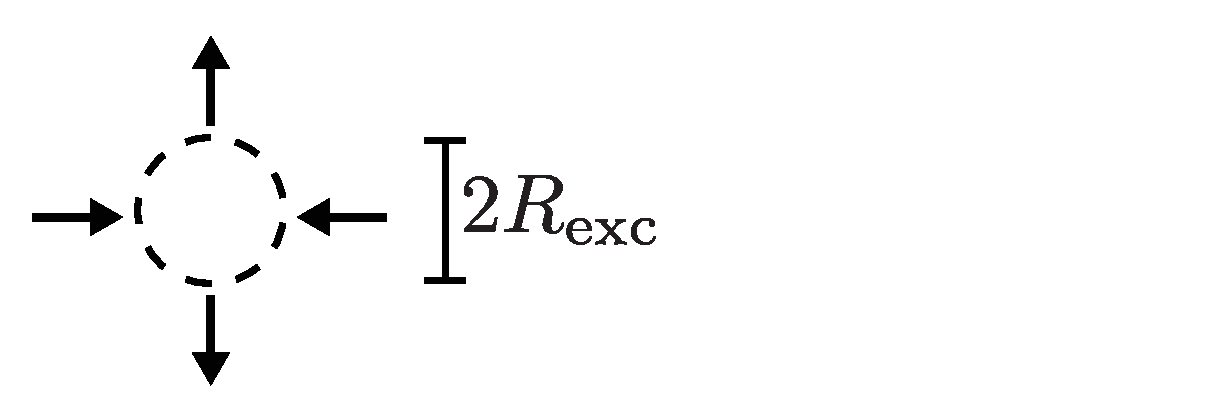
\includegraphics[width=0.75\linewidth]{3.d-kt_geomcharges/chargesequiv-0.pdf}%\caption{Testing}

% \onslide<8>\centering\includegraphics[width=0.75\linewidth]{3.d-kt_geomcharges/chargesequiv-1.pdf}%\caption{Testing}

% %\onslide<8->\centering\includegraphics[width=0.75\linewidth]{3.d-kt_geomcharges/chargesequiv-2.pdf}


% \end{overprint}
    
% \end{figure}
    
% \end{frame}


% \begin{frame}{A Theory of Onset Temperature in 2D: Excitations as a Bound State}
% % \begin{columns}
% % \begin{column}{0.5\linewidth}
% % \begin{itemize}
% %     \item T
% % \end{itemize}
% % \end{column}

% \begin{figure}
% \vspace{-9pt}
% \begin{overprint}
% \onslide<1-10>\centering\includegraphics[width=0.5\linewidth]{3.d-kt_geomcharges/chargesequiv-1.pdf}
% \onslide<11->\centering\includegraphics[width=0.5\linewidth]{3.d-kt_geomcharges/chargesequiv-2.pdf}\hspace{3pt}\raisebox{12pt}{\includegraphics[width=0.35\linewidth]{3.d-kt_geomcharges/dipolemag.pdf}}
% \end{overprint}
% %\begin{equation*}

% %\end{equation*}
% \end{figure}
% \vspace{-7pt}
% % \begin{column}{0.5\linewidth}
% %hint for onset temperature $T_\mathrm{o}$ lies in the mathematical model for the localized pure-shear excitation
% \begin{itemize}
% \item Mathematical analogy (unique to 2D) between elastic defects, i.e., sources of singularities in stress/strain, with multipoles in electrostatics %The free-energy of formation for a localized pure-shear excitation:
% \vspace{8pt}
% \begin{table}[h]
% \begin{tabular}{cc}
% \hline\hline
% Electrostatics  & 2D Elasticity  \\ \hline
% \onslide<2->{Electric field $E_i=-\phi_{,i}$} & \onslide<6->{Stress field $T_{ij} = \chi_{,kk} \delta_{ij}-\chi_{,ij}$}  \\
% \onslide<2->{Potential function $\phi$} & \onslide<7->{Airy stress function $\chi$} \\
% \onslide<3->{Charge distribution $\rho$} & \onslide<8->{Incompatibility source $\eta$}  \\
% \onslide<4->{Dielectric constant $\varepsilon$}    & \onslide<9->{Young's modulus $Y$}   \\
% \onslide<5->{Poisson's equation $-\varepsilon \nabla^2 \phi = \rho$} & \onslide<10->{$\frac{1}{Y} \nabla^4 \chi = \eta$ } \\
% \hline\hline
% \end{tabular}
% %\end{ruledtabular}
% \end{table}
% \vspace{8pt}
% \item<12-> A pure-shear excitation is a bound state of \textbf{geometric dipoles} \pause $ \to$ 2D elastic defects as geometric charges (Moshe, et al. \textit{Proc. Natl. Acad. Sci. U.S.A.} 2015).
% \end{itemize}
% % \end{column}
% % \end{columns}

% \end{frame}
\begin{frame}{A Theory of Onset Temperature in 2D: The Kosterlitz-Thouless Transition}

\begin{columns}[T]
\begin{column}[T]{0.5\textwidth}

\begin{block}{\centering \large Internal Degrees of Freedom}
Excitations have rotation + stretching modes
\end{block}

\begin{figure}
\begin{overprint}
\onslide<2>\centering\includegraphics[width=0.85\linewidth]{c.6-kt_energyentropy/dofs_quadrupole-0.pdf}
\onslide<3>\centering\includegraphics[width=0.85\linewidth]{c.6-kt_energyentropy/dofs_quadrupole-1.pdf}
\onslide<4->\centering\includegraphics[width=0.85\linewidth]{c.6-kt_energyentropy/dofs_quadrupole-3.pdf}
\end{overprint}
\caption{Dipole-pair configurations and internal modes}
\end{figure}

\end{column}

\begin{column}[T]{0.5\textwidth}

\begin{block}{\centering \large The KT Transition}
Critical binding-unbinding condition
\end{block}

\vspace{0.5em}

$$\boxed{\beta_\mathrm{KT} Y^\mathrm{IS} d_\mathrm{c}^2 = 16 \pi}$$

\vspace{0.5em}

\begin{itemize}
\item \textbf{$T < T_\mathrm{KT}$:} Bound dipole pairs $\to$ solid behavior
\item \textbf{$T > T_\mathrm{KT}$:} Free dipoles $\to$ fluid behavior
\item \textbf{Mechanism:} Entropy drives dipole unbinding
\end{itemize}

\vspace{0.5em}

\begin{block}{\centering Connection to KTHNY Theory}
Similar to Kosterlitz-Thouless-Halperin-Nelson-Young theory of dislocation-mediated melting\footnote{Kosterlitz \& Thouless, \textit{J. Phys. C} (1972-73); Halperin \& Nelson, \textit{PRL} (1978); Nelson \& Halperin, \textit{PRB} (1979); Young, \textit{PRB} (1979)}
\end{block}

\end{column}
\end{columns}

\end{frame}
\begin{frame}[t]{A Theory of Onset Temperature in 2D: The KTHNY Melting Scenario}

\begin{figure}
\begin{overprint}

\onslide<2-4>\centering\includegraphics[height=0.675\textheight]{c.7-kt_meltingscenario/mechanism-0.pdf}%\caption{Testing}

\onslide<5->\centering\includegraphics[height=0.675\textheight]{c.7-kt_meltingscenario/mechanism-1.pdf}%\caption{Testing}

%\onslide<4->\centering\includegraphics[width=0.925\linewidth]{slide_13/dofs_quadrupole-3.pdf}
% \begin{columns}
% \begin{column}{0.5\linewidth}
% \begin{itemize}
%     \item T
% \end{itemize}
% \end{column}

% \begin{column}{0.5\linewidth}

\end{overprint}
    
\end{figure}

\vspace{-10pt}

\only<1-7>{
\begin{itemize}
\item<2-> \textbf{$T < T_\mathrm{KT}$:} Rare localized pure-shear excitations \onslide<3->{$\to$ a (defected) solid at intermediate timescales} \onslide<4->{$\to$ \textbf{a renormalized shear modulus} $\km{G^\mathrm{R}} < G^\mathrm{IS}$.}
\item<5-> \textbf{$T > T_\mathrm{KT}$:} Proliferation of free dipoles \onslide<6->{$\to$ \textbf{entropy} drives the system to behave as a fluid}\onslide<7->{$\to$ vanishing renormalized shear modulus $\km{G^\mathrm{R}} =0$}

%\only<6->{$\to$ similar to the Kosterlitz-Thouless-Halperin-Nelson-Young (KTHNY) theory.}
%\footnote{Kosterlitz and Thouless, \textit{J. Phys. C} (1972); Kosterlitz and Thouless, \textit{J. Phys. C} (1973); Halperin and Nelson, \textit{Phys. Rev. Lett.} (1978); Nelson, \textit{Phys. Rev. B} (1978); Nelson and Halperin, \textit{Phys. Rev. B} (1979); Young, \textit{Phys. Rev. B} (1979)}}

\end{itemize}
}
\only<8->{
\begin{block}{\Large \centering The Task}
Determine the temperature $T_\mathrm{KT}$ where $\beta_\mathrm{KT} \km{Y^\mathrm{R}(T=T_\mathrm{KT})} d_\mathrm{c}^2 = 16 \pi$ due to unbinding of localized excitations $\to$ Compare predicted $T_\mathrm{KT}$ to observed the onset temperature $T_\mathrm{o}$!
\end{block}
}

% \end{column}

% \end{columns}


    
\end{frame}
%%% Longer Version
% \begin{frame}[c]
% \frametitle{A Theory of Onset Temperature in 2D: Numerical Results} %$J_\sigma$

% \onslide<1->{\begin{table}[h]
% \begin{tabular}{lccccc}
% \hline\hline
% Glass Former  & Observed$^\ddagger$ $T_\mathrm{o}$  & Predicted (Approximate$^\dagger$) $T_\mathrm{KT}^\mathrm{app}$ & Predicted (RG) $T_\mathrm{KT}$  \\ \hline
% Poly-(12,0), ($\varepsilon=0.2$)  & \tikzmark{start} 0.25  & 0.38 & 0.27 \tikzmark{end}  \\
% Poly-(12,6), ($\varepsilon=0.2$)    & 0.17  & 0.16 & 0.11   \\
% Poly-(18,0), ($\varepsilon=0.0$)    & 1.10  & 2.00 & 1.40   \\
% Poly-(18,0), ($\varepsilon=0.2$)    & 0.39  & 0.51 & 0.35   \\
% Poly-(10,6), ($\varepsilon=0.1$)    & 0.17  & 0.35 & 0.24  \\
% Poly-(10,6), ($\varepsilon=0.2$)    & 0.14  & 0.15 & 0.10   \\
% \hline\hline
% \only<3->{\begin{tikzpicture}[overlay,remember picture]
%   \draw[red, thick] ([shift={(-1ex,2ex)}]pic cs:start) rectangle ([shift={(1ex,-0.5ex)}]pic cs:end);
% \end{tikzpicture}
% }
% \end{tabular}
% \vspace{-12pt}
% \caption{\footnotesize $^\ddagger$ From fitting relaxation time $\tau_\mathrm{eq}$ data. (Fraggedakis, Hasyim, Mandadapu, \texttt{arXiv:2204.07528}, 2022). $^\dagger$ From energy-entropy arguments $\beta \tilde{Y}^\mathrm{IS} d_\mathrm{c}^2 = 16\pi$.}
% %\end{ruledtabular}
% \end{table}
% }
% \vspace{-12pt}
% \begin{itemize}
%     \item<2-> Reasonable agreement is found between observed onset and RG calculation, across all polydisperse glass formers!
%     \item<4-> Prediction based on energy-entropy argument overestimates the true onset temperature $T_\mathrm{o}$
%     %\item<6-> \textbf{Finite-size effects}: MSD scales as $\ln R$ (in 2D), $R$ is the linear system size.
% \end{itemize}

% \onslide<5->{\km{\large{What are the consequences of the KT transition to dynamics at intermediate timescales?}}}

% \end{frame}


%%% Shorter Version
\begin{frame}[c]
\frametitle{A Theory of Onset Temperature in 2D: Numerical Results} %$J_\sigma$

\begin{columns}

\begin{column}{0.55\linewidth}

\onslide<5->{\begin{table}[h]
\begin{tabular}{lccccc}
\hline\hline
Glass Former  & Observed$^\ddagger$ $T_\mathrm{o}$  & RG $T_\mathrm{KT}$  \\ \hline
Poly-(12,0), ($\varepsilon=0.2$)  & \tikzmark{start} 0.25  & 0.27 \tikzmark{end}  \\
Poly-(12,6), ($\varepsilon=0.2$)    & 0.17  & 0.11   \\
Poly-(18,0), ($\varepsilon=0.0$)    & 1.10  & 1.40   \\
Poly-(18,0), ($\varepsilon=0.2$)    & 0.39  & 0.35   \\
Poly-(10,6), ($\varepsilon=0.1$)    & 0.17  & 0.24  \\
Poly-(10,6), ($\varepsilon=0.2$)    & 0.14  & 0.10   \\
2D Kob-Andersen 65:35 & 1.00 & 0.95 \\
\hline\hline
\only<6->{\begin{tikzpicture}[overlay,remember picture]
  \draw[red, thick] ([shift={(-1ex,2ex)}]pic cs:start) rectangle ([shift={(1ex,-0.5ex)}]pic cs:end);
\end{tikzpicture}
}
\end{tabular}
\vspace{-12pt}
\caption{\footnotesize $^\ddagger$ From fitting relaxation time $\tau_\mathrm{eq}$ data (Fraggedakis, Hasyim, Mandadapu, \texttt{arXiv:2204.07528}, 2022). }%$^\dagger$ Using RG calculations. (Fraggedakis, Hasyim, Mandadapu, \texttt{arXiv:2204.07528}, 2022)}
%\end{ruledtabular}
\end{table}
}
\vspace{-12pt}
\begin{itemize}
    \item<1-> There's no closed-form formula for $T_\mathrm{KT}$! 
    \item<4-> Use renormalization group (RG)\footnotemark + elastic and structural properties as input (just like $J_\sigma$).
    %\item<6-> \textbf{Finite-size effects}: MSD scales as $\ln R$ (in 2D), $R$ is the linear system size.
\end{itemize}

\end{column}

\begin{column}{0.45\linewidth}

\begin{overprint}
\onslide<2>\begin{figure}
\vspace{30pt}
$$ \frac{1}{\tilde{Y}^{\mathrm{R}} }= \underbrace{\frac{1}{\tilde{Y}^{\mathrm{IS}}}}_{\substack{\text{Bare shear} \\ \text{modulus}}}+\underbrace{\frac{A_{0}}{d_{\mathrm{c}}^{2}}\left(\left\langle\hat{\epsilon}_{i j}^{\mathrm{e}} \hat{\epsilon}_{i j}^{\mathrm{e}}\right\rangle-\frac{1}{2}\left\langle\hat{\epsilon}_{i i}^{\mathrm{e}} \hat{\epsilon}_{k k}^{\mathrm{e}}\right\rangle\right)}_{\substack{\text{Renormalization due to} \\ \text{dipolar excitations}}} $$
where $\tilde{Y}^\mathrm{R} = \beta Y^\mathrm{R} d_\mathrm{c}^2$ and $\tilde{Y}^\mathrm{IS} = \beta Y^\mathrm{IS} d_\mathrm{c}^2$

\caption{The task entails computing ensemble averages over excitation DOFs.} 

    
\end{figure}

\onslide<3>\begin{figure}
\centering\includegraphics[height=0.675\textheight]{c.8-kt_results_1/new-mechanism-0.pdf}\caption{Melting transition is a \textbf{critical point} $\to$ naive calculations of $Y^\mathrm{R}$ fails (divergent)!}
\end{figure}

\onslide<4->\begin{figure}
\vspace{30pt}
\begin{gather*}
\frac{\mathrm{d} \tilde{Y}^{-1}}{\mathrm{~d} \ell} =\frac{\pi^{2}}{4} \tilde{y}^{2} e^{\frac{\tilde{Y}}{8 \pi}}\left(2 I_{0}\left(\frac{\tilde{Y}}{8 \pi}\right)-I_{1}\left(\frac{\tilde{Y}}{8 \pi}\right)\right) 
\\
\frac{\mathrm{d} \tilde{y}}{\mathrm{~d} \ell} =\left(2-\frac{\tilde{Y}}{8 \pi}\right) \tilde{y}+2 \pi \tilde{y}^{2} e^{\frac{\tilde{Y}}{16 \pi}} I_{0}\left(\frac{\tilde{Y}}{8 \pi}\right) 
\\
\tilde{Y}(0) = \tilde{Y}^\mathrm{IS}; \tilde{y}(0) = e^{-\beta E_\mathrm{c}}
\end{gather*}

where $I_n(x)$ is the $n$-th order modified Bessel function of the first kind

\caption{
RG yields differential equations for renormalized Young's modulus $\tilde{Y}$ and \km{fugacity $\tilde{y}$}.
} 

\end{figure}

\end{overprint}

\end{column}


\end{columns}

\only<4->{\footnotetext{
Nelson and Halperin, \textit{Phys. Rev. B} (1978)
}
}

\end{frame}
\begin{frame}[c]
\frametitle{A Theory of Onset Temperature in 2D: Finite-Size Effects at $T \ll T_\mathrm{o}$
} %$J_\sigma$

\begin{columns}[T]

\begin{column}[T]{0.5\linewidth}

\begin{figure}
\includegraphics[height=0.5\textheight]{c.10-kt_merminwagner_1/merminwagner_comparison_0.pdf}
\caption{MSD at $t=100 \ll \tau_\mathrm{eq}$. (Shiba, Kawasaki, Kim, \textit{PRL}, 2019).  \onslide<3->{$\km{\sigma_\mathrm{MSD} (k,T)= f(T) \frac{k^2}{2} \approx \textbf{0.25}}$}.}
\vspace{-20pt}
\begin{gather*}
    \mathrm{MSD} \sim f(T) \ln R
    \\
    f(T) = k_{\mathrm{B}} T \frac{\left(3-\nu^{\mathrm{R}}\right)\left(1+\nu^{\mathrm{R}}\right)}{2 \pi Y^{\mathrm{R}}}
\end{gather*}
    
\end{figure}
\end{column}

\begin{column}[T]{0.5\linewidth}

\begin{figure}
\includegraphics[height=0.5\textheight]{c.10-kt_merminwagner_1/merminwagner_comparison_1.pdf}
\caption{$F_s(k,t)$ at $t=100 \ll \tau_\mathrm{eq}$ and $k\approx 2\pi$. (Shiba, Kawasaki, Kim, \textit{PRL}, 2019). \onslide<2->{$\km{\sigma(k,T) \approx \textbf{0.26}}$}}
\vspace{-20pt}
    \begin{gather*}
    F_{s}\left(k,t \right)  \sim R^{-\frac{\sigma(k, T)}{2}} \\
    \km{\sigma(k, T)} = k_{\mathrm{B}} T \frac{k^{2}\left(3-\nu^{\mathrm{R}}\right)\left(1+\nu^{\mathrm{R}}\right)}{4 \pi Y^{\mathrm{R}}}
    \end{gather*}
\end{figure}

\end{column}

\end{columns}

\end{frame}

% \begin{frame}[c]
% \frametitle{A Theory of Onset Temperature in 2D: Finite-Size Effects MSD} %$J_\sigma$

% \begin{columns}

% \begin{column}{0.45\linewidth}

% \begin{figure}

% \begin{overprint}
% \onslide<4>\centering\includegraphics[height=0.75\textheight]{8.d-kt_merminwagner/shiba_msd.png}
% \caption{MSD data from MD simulations (Shiba, Kawasaki, Kim, \textit{Phys. Rev. Lett.}, 2019)}

% \onslide<5-6>\centering\includegraphics[height=0.75\textheight]{8.d-kt_merminwagner/shiba_msd_witharrow.pdf}
% \caption{MSD data from MD simulations (Shiba, Kawasaki, Kim, \textit{Phys. Rev. Lett.}, 2019)}

% \onslide<7-9>\centering\includegraphics[height=0.725\textheight]{8.d-kt_merminwagner/msd_merminwagner_0.pdf}
% \caption{Replotting MSD at $t=100$ reveals logarithmic finite-size scaling (Shiba, Kawasaki, Kim, \textit{Phys. Rev. Lett.}, 2019)}

% \onslide<10->\centering\includegraphics[height=0.725\textheight]{8.d-kt_merminwagner/msd_merminwagner_1.pdf}
% \caption{Logarithmic scaling can also be found in other 2D systems (Illing, et al. \textit{Proc. Natl. Acad. Sci. U.S.A.}, 2017)}
% %\onslide<7->\includegraphics[height=0.4\textheight]{example-image-a}
% %}


% \end{overprint}

% \end{figure}

% \end{column}

% \begin{column}{0.55\linewidth}

% \begin{itemize}
%     \item<2-> Supercooled liquids behave as a 2D solid at intermediate timescales ($t \sim \mathcal{O}(\tau_\mathrm{jump})$) 
%     \item<3-> Displacement fluctuations at $t \sim \mathcal{O}(\tau_\mathrm{jump})$ $\leftrightarrow$ elastic fluctuations (\textbf{Mermin-Wagner}) 
%     \item<6->Our theory yields logarithmic scaling:
%     \onslide<6->
%     {\begin{center}
%     \begin{minipage}{0.85\textwidth}
%     \begin{block}{\centering Finite-Size Effects (MSD)}
%     \begin{gather*}
%     \mathrm{MSD} = f(T) \ln \frac{R}{\xi^{*}} \sim \ln R
%     \\
%     f(T) = k_{\mathrm{B}} T \frac{\left(3-\nu^{\mathrm{R}}\right)\left(1+\nu^{\mathrm{R}}\right)}{2 \pi Y^{\mathrm{R}}}
%     \end{gather*}
%     \end{block}
%     \end{minipage}
%     \end{center}
%     }
%     \item<8-> Depends on \textit{renormalized} elastic moduli! 
%     \item<9->$\xi^*(T)$ is a short-distance cut-off identified from the RG analysis ($\xi^*(T) \to O(\sigma_\mathrm{d})$ as $T \to 0$).
% \end{itemize}

% \end{column}

% \end{columns}

% \end{frame}

% \begin{frame}[c]
% \frametitle{A Theory of Onset Temperature in 2D: Finite-Size Effects $F_s(k,t)$} %$J_\sigma$

% \begin{columns}[T]

% \begin{column}[T]{0.45\linewidth}

% \begin{figure}[t]

% \begin{overprint}
% \onslide<3>\centering\vspace{20pt}\includegraphics[width=0.9\linewidth]{8.d-kt_merminwagner/fskt_szamelflenner.png}
% \caption{Relaxation proceeds faster as system size is increased (Flenner and Szamel, \textit{Nat. Comm.}, 2015). 2D KA 68:32 system, $k=2 \pi/\sigma_{A}$}

% \onslide<4>\centering\vspace{20pt}\includegraphics[width=0.9\linewidth]{8.d-kt_merminwagner/fskt_szamelflenner_1.png}
% \caption{Relaxation proceeds faster as system size is increased (Flenner and Szamel, \textit{Nat. Comm.}, 2015). 2D KA 68:32 system, $k=2 \pi/\sigma_{A}$}

% \onslide<5>\centering\includegraphics[height=0.725\textheight]{8.d-kt_merminwagner/fskt_merminwagner_0.pdf}
% \caption{Replotting $F_s(k,t=100)$ reveals power-law finite-size scaling (Flenner and Szamel, \textit{Nat. Comm.}, 2015)}

% \onslide<6-7>\centering\includegraphics[height=0.725\textheight]{8.d-kt_merminwagner/fskt_merminwagner_1.pdf}
% \caption{Other studies have demonstrated this too (Shiba, Kawasaki, Kim, \textit{Phys. Rev. Lett.}, 2019)}

% \onslide<8->\centering\includegraphics[height=0.725\textheight]{8.d-kt_merminwagner/merminwagner_comparison.pdf}
% \caption{We can estimate the scaling exponent $\sigma(k,T)$ for $F_s(k,t)$ from the MSD}
% %\onslide<7->\includegraphics[height=0.4\textheight]{example-image-a}
% %}


% \end{overprint}

% \end{figure}

% \end{column}

% \begin{column}[T]{0.55\linewidth}

% \begin{itemize}
%     \item<1-> Mermin-Wagner fluctuations impact other measures for relaxation, i.e., intermediate scattering function (density fluctuations).
%     \onslide<2->{
%     \begin{center}
%     \begin{minipage}{0.85\textwidth}
%     \begin{block}{\centering Finite-Size Effects ($F_s(k,t)$)}
%     \vspace{-1em}
%     \begin{gather*}
%     F_{s}\left(k,\left\langle\tau_{\mathrm{jump}}\right\rangle\right)  \simeq\left(\frac{R}{\xi^{*}}\right)^{-\frac{\sigma(k, T)}{2}} \\
%     \sigma(k, T) = k_{\mathrm{B}} T \frac{k^{2}\left(3-\nu^{\mathrm{R}}\right)\left(1+\nu^{\mathrm{R}}\right)}{4 \pi Y^{\mathrm{R}}}
%     \end{gather*}
%     \end{block}
%     \end{minipage}
%     \end{center}
%     }
%     \item<7-> Exponent $\sigma(k,T)$ is related to the prefactor $f(T)$ in the MSD:
%     \begin{equation*}
%     \sigma (k,T) = f(T) \frac{k^2}{2}    
%     \end{equation*}
%     \item<9-> From $F_s(k,t)$: $\sigma(k,T) \approx \textbf{0.26}$. 
    
%     \onslide<10->{From MSD: $\sigma(k,T) \approx (1.26 \cdot 10^{-2}) \frac{k^2}{2} \approx  \textbf{0.25}$.} 
% \end{itemize}

% \end{column}

% \end{columns}

% \end{frame}
% \begin{frame}{A Theory of Onset Temperature in 2D: Young's Modulus as $T \to T_\mathrm{KT}$}

% \begin{columns}

% \begin{column}[T]{0.45\textwidth}

% \begin{itemize}
%     \item<2->Pick an intermediate time $\Delta t \ll \tau_\mathrm{eq}$ and measure strain fluctuations at $t = \Delta t$
%     \only<2-3> 
%     {
%     \begin{equation*}
%     \frac{1}{Y^\mathrm{R}} = \beta A_0 \left(\left\langle\hat{\epsilon}_{i j} \hat{\epsilon}_{i j}\right\rangle+\frac{1}{2}\left\langle\hat{\epsilon}_{i i}\hat{\epsilon}_{k k}\right\rangle\right)
%     \end{equation*}
%     }
%     \begin{figure}
%     \begin{overprint}
%     \onslide<4-17>\centering\includegraphics[height=0.65\textheight]{9.d-kt_keim/Yrenorm_poly12.pdf}\caption{The predicted Young's modulus according to RG calculations (discontinuity at $T=T_\mathrm{KT}$)}
    
%     \onslide<18->\centering\includegraphics[height=0.625\textheight]{9.d-kt_keim/msd_poly12.pdf}\caption{MSD Data of Poly-(12,0) around the onset temperature, which is qualitatively similar to experimental data.}
%     \end{overprint}
%     \end{figure}
    
% \end{itemize}

% \end{column}

% \begin{column}[T]{0.5\textwidth}

% \begin{itemize}
%     \item<5-> Similar measurements have been done in an \textit{experimental} study (Klix, Maret, and Keim \textit{Phys. Rev. X} 2015)
%     \begin{figure}
%     \begin{overprint}
%     \onslide<6>\centering\includegraphics[width=\linewidth]{9.d-kt_keim/keim_setup_0.pdf}\caption{A colloidal system (polystyrene spheres) confined to a flat water-air interface (Ebert, et.al. \textit{Rev. Sci. Instrum} 2009).}
%     \onslide<7>\centering\includegraphics[width=\linewidth]{9.d-kt_keim/keim_setup_1.pdf}\caption{A colloidal system (polystyrene spheres) confined to a flat water-air interface (Ebert, et.al. \textit{Rev. Sci. Instrum} 2009).}
%     \onslide<8>\centering\includegraphics[width=\linewidth]{9.d-kt_keim/keim_setup_1.pdf}\caption{Each sphere is doped with magnetite}
%     \onslide<9-10>\centering\includegraphics[width=\linewidth]{9.d-kt_keim/keim_setup_2.pdf}\caption{Each sphere is doped with magnetite $\to$ tuning of pair dipolar interaction between particles}\onslide<10>{$$\km{ \text{Coupling strength} \ \Gamma} \sim \beta H^2 $$}
%     \onslide<11>\centering\includegraphics[height=0.6\textheight]{9.d-kt_keim/keim_screenshot.png}\caption{Bulk and shear moduli data at different $\Gamma$ values  (Klix, Maret, and Keim \textit{Phys. Rev. X} 2015).}
%     \onslide<12>\raggedright\vspace{15pt}{\textit{Concerning the height of the jumps, we are not aware of predictions of universal behavior of elasticity in thermal amorphous systems as, e.g., the famous $16 \pi \approx 50.26$ for Young's modulus in $2 \mathrm{D}$ melting [40], but the measured values in glass and crystal are of} \textbf{the same order.} 
%     \vspace{5pt}
    
%     \hfill ---- Klix, Maret, and Keim \textit{Phys. Rev. X} 2015}
%     \onslide<13>\centering\includegraphics[height=0.6\textheight]{9.d-kt_keim/youngmodulus_keim_0.pdf}\caption{Young's modulus data, (re)computed from the bulk/shear moduli data.}
%     \onslide<14>\centering\includegraphics[height=0.6\textheight]{9.d-kt_keim/youngmodulus_keim_1.pdf}\caption{Young's modulus data, (re)computed from the bulk/shear moduli data.}
%     \onslide<15>\centering\includegraphics[height=0.6\textheight]{9.d-kt_keim/youngmodulus_keim_2.pdf}\caption{Young's modulus data, (re)computed from the bulk/shear moduli data.}
%     \onslide<16>\centering\includegraphics[width=0.9\linewidth]{9.d-kt_keim/msd_keim.png}\caption{Their MSD data around the transition  (Klix, Maret, and Keim \textit{Phys. Rev. X} 2015).}
%     \onslide<17->\centering\includegraphics[width=0.9\linewidth]{9.d-kt_keim/msd_keim_1.png}\caption{Their MSD data indicates that the transition is occurring near the onset point for glassy dynamics  (Klix, Maret, and Keim \textit{Phys. Rev. X} 2015).}
%     \end{overprint}
%     \end{figure}
% \end{itemize}


% \end{column}

% \end{columns}  
% \end{frame}

\begin{frame}{A Theory of Onset Temperature in 2D: Young's Modulus as $T \to T_\mathrm{KT}$}

%\vspace{15pt}

\begin{columns}

\begin{column}[T]{0.425\textwidth}

\begin{figure}
    \begin{overprint}
    \onslide<4-5>\centering\includegraphics[height=0.65\textheight]{9.d-kt_keim/Yrenorm_poly12.pdf}\caption{The predicted Young's modulus according to RG calculations (discontinuity at $T=T_\mathrm{KT}$)}
    
    \onslide<6>\vspace{15pt}\centering\includegraphics[width=\linewidth]{9.d-kt_keim/keim_setup_0.pdf}\caption{A colloidal system (polystyrene spheres) confined to a flat water-air interface (Ebert, et.al. \textit{Rev. Sci. Instrum} 2009).}
    
    \onslide<7>\vspace{15pt}\centering\includegraphics[width=\linewidth]{9.d-kt_keim/keim_setup_1.pdf}\caption{A colloidal system (polystyrene spheres) confined to a flat water-air interface (Ebert, et.al. \textit{Rev. Sci. Instrum} 2009).}
    
    \onslide<8>\vspace{15pt}\centering\includegraphics[width=\linewidth]{9.d-kt_keim/keim_setup_1.pdf}\caption{Each sphere is doped with magnetite}
    
    \onslide<9-10>\vspace{15pt}\centering\includegraphics[width=\linewidth]{9.d-kt_keim/keim_setup_2.pdf}\caption{Each sphere is doped with magnetite $\to$ tuning of pair dipolar interaction between particles}
    
    \onslide<11>\centering\includegraphics[height=0.65\textheight]{9.d-kt_keim/YRG_keim_exp_0.pdf}\caption{Young's modulus data, (re)computed from the bulk/shear moduli data.}
    
    \onslide<12>\raggedright\vspace{30pt}{\textit{Concerning the height of the jumps, we are not aware of predictions of universal behavior of elasticity in thermal amorphous systems as, e.g., \km{the famous $16 \pi \approx 50.26$ for Young's modulus in $2 \mathrm{D}$ melting} [40], but the measured values in glass and crystal are of} \textbf{the same order.} 
    \vspace{5pt}
    
    -- Klix, Maret, and Keim, \textit{PRX} 2015}
    

    \onslide<13>\centering\includegraphics[height=0.65\textheight]{9.d-kt_keim/YRG_keim_exp_1.pdf}\caption{Young's modulus data, (re)computed from the bulk/shear moduli data.}
    
    \onslide<14>\centering\includegraphics[height=0.65\textheight]{9.d-kt_keim/YRG_keim.pdf}\caption{Prediction agrees with experiments. Input: RDF and Young's modulus at high-$\Gamma$\vspace{-10pt}\footnote{ F. Ebert, Ph.D. Dissertation, 2008; C. Klix, Ph.D. Dissertation, 2014}.}
    
    \onslide<15>\centering\includegraphics[height=0.75\textheight]{9.d-kt_keim/YRG_keim_closeup.pdf}\caption{A closeup of RG prediction with exp. data}
    
    \onslide<16>\vspace{20pt}\centering\includegraphics[width=\linewidth]{9.d-kt_keim/msd_keim.png}\caption{MSD data around the transition  (Klix, Maret, and Keim \textit{Phys. Rev. X} 2015).}
    
    \onslide<17>\vspace{20pt}\centering\includegraphics[width=\linewidth]{9.d-kt_keim/msd_keim_1.png}\caption{MSD data indicates that the transition is occurring near the onset point for glassy dynamics  (Klix, Maret, and Keim \textit{Phys. Rev. X} 2015).}
    
    % \onslide<19>\vspace{15pt}\centering\includegraphics[width=\linewidth]{9.d-kt_keim/msd_poly12.pdf}\caption{MSD Data of Poly-(12,0) around $T_\mathrm{o}$ is qualitatively similar to experimental data.}
    
    \onslide<18->\centering\includegraphics[height=0.75\textheight]{9.d-kt_keim/YRG_keim_closeup.pdf}%\caption{MSD Data of Poly-(12,0) around $T_\mathrm{o}$ is qualitatively similar to experimental data.}
    
    
    \end{overprint}
    \end{figure}
    

\end{column}

\begin{column}[T]{0.575\textwidth}


\begin{itemize}
    \item<2->Pick an intermediate time $\Delta t \ll \tau_\mathrm{eq}$ and measure strain fluctuations at $t = \Delta t$:
    \begin{equation*}
    \frac{1}{Y^\mathrm{R}} = \beta A_0 \left(\left\langle\hat{\epsilon}_{i j} \hat{\epsilon}_{i j}\right\rangle+\frac{1}{2}\left\langle\hat{\epsilon}_{i i}\hat{\epsilon}_{k k}\right\rangle\right)
    \end{equation*}
    \item<5-> Similar measurements have been done in an \textit{experimental} study (Klix, Maret, and Keim \textit{Phys. Rev. X} 2015)
    \onslide<10->{$${ \text{\textbf{Coupling strength}} \ \bm \Gamma} \sim \beta H^2 $$}
    \vspace{-18pt}
    \item<14-> Apply the RG theory given existing data available from Keim and Maret group.
    \onslide<18->\begin{block}{\centering Inherent-State Melting as a "Hidden" Transition}
    \vspace{5pt}
    \centering The mechanism is thermodynamic in character but observable dynamically at $t \ll \tau_\mathrm{eq}(T)$
    \vspace{5pt}
    \end{block}

\end{itemize}


\end{column}

\end{columns}  
\end{frame}
\begin{frame}[c]
\frametitle{A Theory of Onset Temperature in 2D: Spatial Correlations} %$J_\sigma$

\begin{columns}[T]

\begin{column}[T]{0.45\linewidth}

\begin{figure}[t]
\begin{overprint}
    \onslide<5->\centering\includegraphics[height=0.75\textheight]{10.d-kt_spatialcorrel/spatialcorrel.pdf}\caption{Predicted spatial correlations for Poly-(12,0) $\varepsilon=0.2$. High-$T$ correlations decay exponentially.}
    %\onslide<5>\centering\includegraphics[height=0.675\textheight]{2.d-kt_thermoframework/Energy_Landcape_Voronoi.png}\caption{Testing a sentence that I want to write which will be this long}
\end{overprint}
\end{figure}

\end{column}

\begin{column}{0.55\linewidth}

\begin{itemize}
    \item<1-> The only major unverified prediction left is on \textit{spatial correlations}. \onslide<2->{Let $\rho_{\* k}( \* x,t) = e^{i \*k \cdot \* u(\* x, t)}$ be an order parameter.}
    \item<3-> Our theory predicts power-law decay:
    \onslide<4->{
    \begin{center}
    \begin{minipage}{0.85\textwidth}
    \begin{block}{\centering Low-$T$ Spatial Correlations}
    \vspace{-1em}
    \begin{align*}
    C_{\mathbf{k}}\left(\mathbf{x},\left\langle\tau_{\text {jump }}\right\rangle\right) &:= \left\langle\rho_{\mathbf{k}}\left(\mathbf{x},\left\langle\tau_{\text {jump }}\right\rangle\right) \rho_{-\mathbf{k}}(\mathbf{0}, 0)\right\rangle \\
     &\simeq\left(\frac{|\mathbf{x}|}{R}\right)^{-\sigma(k, T)}
     \\
    \sigma(k, T) &= k_{\mathrm{B}} T \frac{k^{2}\left(3-\nu^{\mathrm{R}}\right)\left(1+\nu^{\mathrm{R}}\right)}{4 \pi Y^{\mathrm{R}}}
    \end{align*}
    \end{block}
    \end{minipage}
    \end{center}
    }
    \item<6-> Testable by measuring displacement fluctuations at intermediate timescales but requires enormous system sizes to resolve (\textbf{future work})
\end{itemize}

\end{column}

\end{columns}

\end{frame}

% Part D: Facilitation Theory

\begin{frame}\label{d.1}
\frametitle{A Theory of Dynamical Facilitation: General Idea}

\begin{columns}[T]
\begin{column}[T]{0.5\textwidth}

\begin{figure}[t]
%\includegraphics[height=0.65\textheight]{figures/pel_hopping.png}
\begin{overprint}
\vspace{-10pt}
\onslide<2>\includegraphics[width=0.975\linewidth]{1.c-fac_intro/interlude1.pdf}\caption{So far, we only discuss the first hopping event!}

\onslide<3>\includegraphics[width=0.975\linewidth]{1.c-fac_intro/interlude2.pdf}\caption{Relaxation involves traversing a series of ISs and energy barriers.}

\onslide<4>\includegraphics[width=0.95\linewidth]{1.c-fac_intro/bare_test_0.pdf}\vspace{-10pt}\caption{A system always begins with no excitations.}

\onslide<5-6>\includegraphics[width=0.95\linewidth]{1.c-fac_intro/bare_test_3.pdf}\vspace{-10pt}\caption{More excitations are created over time, anywhere in space.}

\onslide<7>\includegraphics[width=0.95\linewidth]{1.c-fac_intro/test_3.pdf}\vspace{-10pt}\caption{Excitations leave behind \textbf{elastic fields}.}

\onslide<8->\includegraphics[width=0.95\linewidth]{1.c-fac_intro/test_6.pdf}\vspace{-10pt}\caption{Elastic fields continue to accumulate until full relaxation is reached}

\end{overprint}
\end{figure}

\end{column}

\begin{column}[T]{0.5\textwidth}
\vspace{-12pt}
\begin{block}{\centering \large Origin of Facilitation}
\centering Excitations alter energy barriers for relaxation via elasticity.
{\footnotesize (Hasyim, Mandadapu,  \texttt{arXiv:2310.06584} 2023)}
%(Hasyim, Mandadapu,  \textit{J. Chem. Phys.} 155, 044504 (2021))
\end{block}

\begin{itemize}
    \item<2->Barrier for first excitation is 
    \begin{equation*}
    J_\sigma = G^\mathrm{IS} (\pi R_\mathrm{exc})^2 \epsilon_\mathrm{c}^2
    \end{equation*}
    \item<9-> Energy barrier includes interaction with the accumulated stress:
    \only<10->{
    \begin{gather*}
    J_\sigma\onslide<11->{+\km{\int \diff^2 \* x \ T_{ij}^\alpha d_{ij}^\ddagger}}
    \\
    \onslide<12->
    {d_{ij}^\ddagger: \ \text{the shear strain of the new excitation.}
    }
    \\
    \onslide<13->{T_{ij}^\alpha: \ \text{Stress at the current IS (labeled $\alpha$).}
    }
    \end{gather*}
    }
\end{itemize}

\end{column}
\end{columns}

\end{frame}

\begin{frame}
\frametitle{A Theory of Dynamical Facilitation: Technical Summary}

\begin{enumerate}
    \item<1-> Glassy dynamics via a master equation, governing a hopping process from IS $\alpha$ to another IS $\alpha^\prime$:
    \begin{gather*}
    \frac{\diff p_\alpha(t)}{\diff t} = \sum_{\alpha^\prime} w_{\alpha \alpha^\prime} p_{\alpha^\prime}(t) - w_{\alpha^\prime \alpha}p_\alpha(t) \,, 
    %\begin{equation}
    \quad w_{\alpha^\prime \alpha } = \nu_\mathrm{0} e^{-\beta \Delta F_{\alpha^\prime \alpha}^\ddagger} \,. %\label{eq:transitionrate} \label{eq:mastereq}
    \end{gather*}
    \item<2-> Energy barrier to create a new excitation (labeled $\mu$) is based on elasticity theory:
    %The stress interaction term becomes a pair potential
    %:
    \begin{gather*}
    \Delta F_{\alpha^\prime \alpha}^\ddagger = J_\sigma + \km{\sum_{\mu \prime \neq \mu} v_\mathrm{int}^{\mu  \mu^\prime}} \only<3->{\,, \quad  v^{\mu \mu^\prime}_\mathrm{int} =
    \frac{4\km{\kappa}J_\sigma R_\mathrm{exc}^2}{(r^{\mu \mu^\prime})^2} \cos \left( 2\psi^\mu+2\psi^{\mu^\prime}-4\theta^{\mu \mu^\prime} \right) \,.
    }
    \\
    \only<3->{\km{\kappa \ :} \ \text{interaction strength parameter}}
    \end{gather*}
    \only<3>{
    \centering\includegraphics[width=0.5\linewidth]{2.c-fac_intrc/excconfig2.pdf}
    }
    \only<4>{
    \centering\includegraphics[width=0.6\linewidth]{3.c-fac_results/minima.pdf}
    }
    \item<5-> \textbf{Reversibility:} The energy barrier to create an excitation ($\alpha \to \alpha^\prime$) is the same as reverting the same excitation ($\alpha^\prime \to \alpha$):
    \onslide<6->{
    \begin{equation*}
    \Delta F_{\alpha \alpha^\prime}^\ddagger = \Delta F_{\alpha^\prime \alpha}^\ddagger \only<5->{\  \centering\includegraphics[valign=c,width=0.425\linewidth]{2.c-fac_intrc/pes.pdf}}
    \end{equation*}
    }
    %\begin{figure}
    
    %\end{figure}
    % Given excitation $\mathrm{State} \ 0 \to 1$: Excitation emerges when crossing the first transition state
    % \begin{equation*}
    % \onslide<3->{\Delta F^\ddagger_{10} = J_\sigma}
    % \end{equation*}
    % \item<4-> Excitation leaves behind \textbf{mechanical stress $T_{ij}^1(\* x-\* q^\mu; \psi^\mu)$}
    % \item<5-> $\mathrm{State} \ 1 \to 2$: Second excitation emerges in the presence of previous excitation:
    % \onslide<6->{
    % \begin{equation*}
    % \Delta F^\ddagger_{21} = J_\sigma+\km{\int \diff^2 \* x \ T_{ij}^1 d_{ij}^\ddagger }
    % \end{equation*}
    %}
\end{enumerate}

% \begin{columns}[T]
% \begin{column}[T]{0.5\textwidth}

% \begin{figure}[t]
% %\includegraphics[height=0.65\textheight]{figures/pel_hopping.png}
% \begin{overprint}
% \vspace{12pt}
% \onslide<2>\includegraphics[width=\linewidth]{2.c-fac_intrc/excconfig1.pdf}%\caption{Excitation configuration for the state 1 $\to$ 2 transition.}
% \onslide<3-8>\includegraphics[width=\linewidth]{2.c-fac_intrc/excconfig2.pdf}\only<3-6>{
% \small
% \begin{align*}
% \* q^{\mu \mu^\prime} = \* q^\mu -\* q^{\mu^\prime}: & \ \text{pairwise distance vector}
% \\
% \onslide<4->{q^{\mu \mu^\prime} = \left|\* q^{\mu \mu^\prime}\right|: & \ \text{magnitude of $\* q^{\mu \mu^\prime}$}
% \\
% \theta^{\mu \mu^\prime}: & \ \text{polar angle of $\* q^{\mu\mu^\prime}$}
% \\
% \sigma_\mathrm{exc}: & \ \text{excitation diameter}
% \\
% \km{\kappa}: & \ \text{interaction strength}
% }
% \end{align*}
% }%
% \only<7->{
% \begin{center}
% \begin{block}{\centering Important Note}
% At low temperatures, minima of $v_\mathrm{int}^{\mu \mu^\prime}$ yield most probable excitation \onslide<11->{$\to$ excitation facilitates excitations!}
% \end{block}
% \end{center}
% }

% \onslide<9>\includegraphics[width=\linewidth]{2.c-fac_intrc/bestprofile1.pdf}
% \begin{center}
% \begin{block}{\centering Important Note}
% At low temperatures, minima of $v_\mathrm{int}^{\mu \mu^\prime}$ yield most probable excitation \onslide<11->{$\to$ excitation facilitates excitations!}
% \end{block}
% \end{center}

% \onslide<10->\includegraphics[width=\linewidth]{2.c-fac_intrc/bestprofile.pdf}
% \begin{center}
% \begin{block}{\centering Important Note}
% At low temperatures, minima of $v_\mathrm{int}^{\mu \mu^\prime}$ yield most probable excitation \onslide<11->{$\to$ excitation facilitates excitations!}
% \end{block}
% \end{center}

% \end{overprint}
% \end{figure}


% \end{column}

% \begin{column}[T]{0.5\textwidth}

% \end{column}
% \end{columns}

\end{frame}
% \begin{frame}
% \frametitle{A Theory of Dynamical Facilitation: Summary}

% \begin{columns}[T]
% \begin{column}[T]{0.5\textwidth}

% \begin{figure}[t]
% %\includegraphics[height=0.65\textheight]{figures/pel_hopping.png}
% \begin{overprint}
% \vspace{12pt}
% \onslide<2>\includegraphics[width=\linewidth]{2.c-fac_intrc/excconfig1.pdf}%\caption{Excitation configuration for the state 1 $\to$ 2 transition.}
% \onslide<3-8>\includegraphics[width=\linewidth]{2.c-fac_intrc/excconfig2.pdf}\only<3-6>{
% \small
% \begin{align*}
% \* q^{\mu \mu^\prime} = \* q^\mu -\* q^{\mu^\prime}: & \ \text{pairwise distance vector}
% \\
% \onslide<4->{q^{\mu \mu^\prime} = \left|\* q^{\mu \mu^\prime}\right|: & \ \text{magnitude of $\* q^{\mu \mu^\prime}$}
% \\
% \theta^{\mu \mu^\prime}: & \ \text{polar angle of $\* q^{\mu\mu^\prime}$}
% \\
% \sigma_\mathrm{exc}: & \ \text{excitation diameter}
% \\
% \km{\kappa}: & \ \text{interaction strength}
% }
% \end{align*}
% }%
% \only<7->{
% \begin{center}
% \begin{block}{\centering Important Note}
% At low temperatures, minima of $v_\mathrm{int}^{\mu \mu^\prime}$ yield most probable excitation \onslide<11->{$\to$ excitation facilitates excitations!}
% \end{block}
% \end{center}
% }

% \onslide<9>\includegraphics[width=\linewidth]{2.c-fac_intrc/bestprofile1.pdf}
% \begin{center}
% \begin{block}{\centering Important Note}
% At low temperatures, minima of $v_\mathrm{int}^{\mu \mu^\prime}$ yield most probable excitation \onslide<11->{$\to$ excitation facilitates excitations!}
% \end{block}
% \end{center}

% \onslide<10->\includegraphics[width=\linewidth]{2.c-fac_intrc/bestprofile.pdf}
% \begin{center}
% \begin{block}{\centering Important Note}
% At low temperatures, minima of $v_\mathrm{int}^{\mu \mu^\prime}$ yield most probable excitation \onslide<11->{$\to$ excitation facilitates excitations!}
% \end{block}
% \end{center}

% \end{overprint}
% \end{figure}


% \end{column}

% \begin{column}[T]{0.5\textwidth}

% \begin{itemize}
%     \item<1-> Glassy dynamics as a Markov process, hopping from IS $\alpha$ to another IS $\alpha^\prime$:
    
%     \onslide<2->{(1) Excitation with orientation $\psi^\mu$ and position $\* q^\mu$}\onslide<3->{, and (2) excitation $\psi^{\mu^\prime}$ and position $\* q^{\mu^\prime}$.}
%     \item<4-> The stress interaction term becomes a pair potential%:
%     \onslide<5->{\begin{equation*}
%     v^{\mu \mu^\prime}_\mathrm{int} =
%     \frac{\km{\kappa}J_\sigma \sigma_\mathrm{exc}^2}{(q^{\mu \mu^\prime})^2} \cos \left( 2\psi^\mu+2\psi^{\mu^\prime}-4\theta^{\mu \mu^\prime} \right) %\label{eq:intterm}
%     \end{equation*}
%     }
%     \item<6->  $\mathrm{State} \ 1 \to 2$: $\Delta F_{12}^\ddagger = J_\sigma+v^{21}_\mathrm{int}$
%     %for $\tilde{q}^{\mu \mu^\prime}:= \frac{q^{\mu \mu^\prime}}{\sigma_\mathrm{exc}} \geq 1$ and $v^{\mu \mu^\prime}_\mathrm{int} = \infty$ otherwise.
%     \item<8-> Minimizing $v^{21}_\mathrm{int}$ yields
%     \begin{equation*}
%     \psi^{2*} = 2\theta^{21*}+\pi \left(n+\frac{1}{2}\right) -\psi^1, \ \ \tilde{q}^{21*} = 1  %\label{eq:fminima12}
%     \end{equation*}
%     where $n$ is an integer.
    
%     % Given excitation $\mathrm{State} \ 0 \to 1$: Excitation emerges when crossing the first transition state
%     % \begin{equation*}
%     % \onslide<3->{\Delta F^\ddagger_{10} = J_\sigma}
%     % \end{equation*}
%     % \item<4-> Excitation leaves behind \textbf{mechanical stress $T_{ij}^1(\* x-\* q^\mu; \psi^\mu)$}
%     % \item<5-> $\mathrm{State} \ 1 \to 2$: Second excitation emerges in the presence of previous excitation:
%     % \onslide<6->{
%     % \begin{equation*}
%     % \Delta F^\ddagger_{21} = J_\sigma+\km{\int \diff^2 \* x \ T_{ij}^1 d_{ij}^\ddagger }
%     % \end{equation*}
%     %}
% \end{itemize}

% \end{column}
% \end{columns}

% \end{frame}

\begin{frame}\label{d.4}
\frametitle{A Theory of Dynamical Facilitation: Dynamical Heterogeneity}
\ 
\begin{columns}[T]
\begin{column}[T]{0.5\textwidth}
\centering \only<1>{$\beta J_\sigma = 5$ (Low-T) Displacement Field}
\centering \only<2->{Two-Component Lennard Jones Fluid, $T = 0.5 T_\mathrm{o}$ vs. $\beta J_\sigma = 5$ (Low-T) Displacement Field}
\begin{figure}[t]
\begin{overprint}
\onslide<1>\centering\includemedia[height=0.675\textheight,passcontext,transparent, addresource=d.4-fac_results_1/displowT.mp4, flashvars={source=d.4-fac_results_1/displowT.mp4}]{\includegraphics[height=0.675\textheight]{d.4-fac_results_1/displowT3.png}}{VPlayer.swf}

\onslide<2->\centering\includegraphics[width=\linewidth]{d.4-fac_results_1/out-700.pdf}

\only<2->{\vspace{-2pt}\footnotesize $^1$A. Keys, et al. \textit{Phys. Rev. X} (2011)}
   
\end{overprint}

\end{figure}

\end{column}

\begin{column}[t]{0.5\textwidth}
%\only<2>{Binary Lennard-Jones Fluid, $T = 0.55 T_\mathrm{o}$$^1$}
\centering \only<3>{$\beta J_\sigma = 5$ (Low-T) Persistence Field}
\centering \only<4->{Polydisperse Lennard Jones Fluid, $T = 0.36 T_\mathrm{o}$ vs. $\beta J_\sigma = 5$ (Low-T) Persistence Field}
\begin{figure}[t]
\begin{overprint}
\onslide<3>\centering\includemedia[height=0.675\textheight,passcontext,transparent, addresource=d.4-fac_results_1/persistlowT.mp4, flashvars={source=d.4-fac_results_1/persistlowT.mp4}]{\includegraphics[height=0.675\textheight]{d.4-fac_results_1/persistlowT3.png}}{VPlayer.swf}\onslide<4>{\caption{\textbf{Poisson + cluster point process}}}

%\onslide<4>\centering\includegraphics[height=0.675\textheight]{d.4-fac_results_1/persistlowT3.png}\caption{\textbf{Poisson + cluster point process}}

\onslide<4->\centering\includegraphics[width=0.98\linewidth]{d.4-fac_results_1/persout-012.pdf}

\only<4->{\vspace{-2pt}\footnotesize $^2$B. Guiselin, et al. \textit{Phys. Rev. X} (2022)}

%\centering\includemedia[height=0.675\textheight,passcontext,transparent, addresource=d.4-fac_results_1/movieT009long.mp4, flashvars={source=d.4-fac_results_1/movieT009long.mp4}]{\includegraphics[height=0.675\textheight]{d.4-fac_results_1/persout-012.jpg}}{VPlayer.swf}
\end{overprint}
\end{figure}
\end{column}
\end{columns}
\centering\only<5->{\vspace{-50pt}\Large \textbf{The model displays emergent facilitation!}}
\end{frame}

\begin{frame}{A Theory of Dynamical Facilitation: Emergent Glassy Dynamics}\label{d.5}
\begin{figure}
\begin{overprint}
    \onslide<1>\centering\includegraphics[width=0.85\linewidth]{d.5-fac_results_2/surveyresults1.pdf}
    \onslide<2>\centering\includegraphics[width=0.85\linewidth]{d.5-fac_results_2/surveyresults2.pdf}
    \onslide<3>\centering\includegraphics[width=0.85\linewidth]{d.5-fac_results_2/surveyresults3.pdf}
    \onslide<4>\centering\includegraphics[width=0.85\linewidth]{d.5-fac_results_2/surveyresults.pdf}

\end{overprint}
\end{figure}    
\end{frame}

\begin{frame}\label{d.6}
\frametitle{A Theory of Dynamical Facilitation: \onslide<2->{The Role of Phonons}}

\begin{columns}[T]
\begin{column}[T]{0.5\textwidth}
\begin{figure}
\begin{overprint}
\onslide<2-4>\vspace{20pt}\centering\includegraphics[width=\linewidth]{d.6-fac_results_3/pes.pdf}
\caption{Motion not only consists of hopping (excitations) but also vibrations around minima (phonons).}

\onslide<5>\centering\includegraphics[valign=c,width=0.9\linewidth]{d.6-fac_results_3/newmsdphonons0.pdf}
\caption{Combining analytical formula for phonons with kMC data yields the classic MSD of supercooled liquids!}


\onslide<6>\centering\includegraphics[valign=c,width=0.9\linewidth]{d.6-fac_results_3/ismsdmd.pdf}
\caption{The excitation part of the MSD matches with inherent structure MSD from MD simulations (Shiraishi, et al. \textit{PNAS} (2023)).}

\onslide<8->\centering\includegraphics[valign=c,width=0.9\linewidth]{d.6-fac_results_3/newmsdphonons1.pdf}
\caption{Combining analytical formula for phonons with kMC data yields the two-stage decay in $F_\mathrm{s}(\* k,t))$. Green is the ballistic limit.}

% \onslide<6>\centering\includegraphics[valign=c,width=0.9\linewidth]{d.6-fac_results_3/fsktka.png}
% \caption{The two-stage decay in $F_\mathrm{s}(\*k,t)$ is another classic behavior!}
%\caption{Bond-order autocorrelation function $C_\mathrm{b}(t)$ at high temperatures. $\tau_\mathrm{arr} \sim e^{\beta J_\sigma}$.}    


\end{overprint}
\end{figure}

\end{column}


\begin{column}[t]{0.5\textwidth}
\vspace{-12pt}
\onslide<3->{
\begin{block}{\centering Combining Excitations and Phonons}
\centering As $T \to 0$, phonons and excitations are \textbf{uncorrelated} due to the separation of timescales.  
\end{block}
}
\begin{itemize}
    \item<4-> \textbf{Mean-Squared Displacement:} Add the contributions:
    \begin{equation*}
    \mathrm{MSD}=\mathrm{MSD}_\mathrm{ph}+\mathrm{MSD}_\mathrm{exc}
    \end{equation*}
    %\item<4-> 
    \item<7-> \textbf{Intermediate Scattering Function:} Product of the two contributions
    \begin{gather*}
    F_\mathrm{s}(\*k,t) = F^\mathrm{ph}_\mathrm{s}(\* k,t) F^\mathrm{exc}_\mathrm{s}(\* k,t)
    \\
    F^\mathrm{ph}_\mathrm{s}(\* k,t) = e^{-\frac{k^2}{4}\mathrm{MSD}^\mathrm{ph}(t)}
    \end{gather*}
    %\item<6-> The two-stage decay in $F_\mathrm{s}(\*k,t)$ is another classic behavior!
    % \item<5-> \textbf{Bond-order Autocorrelation Function:} Product of the two contributions
    % \begin{gather}
    % C_\mathrm{b}(t) = C_\mathrm{b}^\mathrm{ph}(t) C^\mathrm{exc}_\mathrm{b}(t)
    % \end{gather}
    
\end{itemize} 

\end{column}

\end{columns}

\end{frame}


% Part E: Conclusion
\begin{frame}\label{e.1}
\frametitle{Acknowledgements}

\begin{columns}[T]

\begin{column}[T]{0.3\textwidth}
\vspace{5pt}
\onslide<2->{\begin{figure}
    \centering
    \includegraphics[width=0.825\linewidth]{acknowledgements/index.jpg}
    \caption{\centering \footnotesize{ \textbf{Advisor:} Kranthi K. Mandadapu  }}
    %\textbf{Co-workers:} Dimitrios Fraggedakis, Sanggeun Song}}
    %\\
    %\textbf{Paper:} \footnotesize } %
    \centering\includegraphics[width=0.8\linewidth]{acknowledgements/image912.png}
    \caption{\centering  \footnotesize{ \textbf{Funding:} DOE, Office of Basic Energy Sciences, Contract No. DEAC02-05CH11231}}
\end{figure}
}
\end{column}

\begin{column}[T]{0.7\textwidth}

\begin{figure}
    \centering\includegraphics[height=0.55\textheight]{a.2-intro_dftheory/DF_Theory_Excitations_Zoom_2.pdf}
    \hspace{1em}
    \centering\includegraphics[height=0.55\textheight]{d.6-fac_results_3/persistlowT3.png}
    
    \caption{A self-consistent model of glassy dynamics based on excitations and elasticity $\to$ excitation-driven glassy dynamics. Future work: \textbf{3D} %, \textbf{Radius of Gyration}.
    \onslide<3->{\textbf{Paper:} M.R. Hasyim, K.K. Mandadapu,  \textit{J. Chem. Phys.} 155, 044504 (2021); M.R. Hasyim, K.K. Mandadapu, \texttt{arXiv:2310.06584} (2023)}
    }
\end{figure}
\vspace{-1.0em}
% D. Fraggedakis, M,R. Hasyim, K.K. Mandadapu.  120.14 \textit{Proc. Natl. Acad. Sci. U.S.A.} (2023); 
%\vspace{20em}
\onslide<4->{\vspace{-0.5em}\Huge \textbf{Questions?}}%e-mail at \texttt{muhammad\_hasyim@berkeley.edu}}
\end{column}

\end{columns}
\end{frame}

\begin{frame}
\frametitle{A Theory of Dynamical Facilitation: The Role of Revertibility}

\begin{columns}[T]
\begin{column}[T]{0.6\textwidth}
\centering $\beta J_\sigma = 1$ (High-T)
\begin{figure}[t]

\begin{overprint}
\onslide<2-3>\centering\includegraphics[width=0.825\textheight]{d.6-fac_results_3/persistlowT.jpg}

\onslide<4->\centering\includegraphics[height=0.7\textheight]{d.1-fac_intro/taubwithirrev.pdf}\caption{Relaxation time data when revertibility is turned off (red markers) along with an Arrhenius timescale $\tau_\mathrm{arr} \sim e^{\beta J_\sigma}$.}

\end{overprint}

\end{figure}
\end{column}

\begin{column}[t]{0.4\textwidth}

\begin{block}{\centering Origin of Glassy Behavior}
\centering A combination of \textbf{emergent constraints} and \textbf{revertibility} of dynamics. 
\end{block}

\begin{enumerate}
   \item<2-> \textbf{Emergent Constraints:} Dynamics only persist in a few spots of the liquid. 
   \item<3-> \textbf{Revertibility:} Within an active region, excitations can go back and forth, wasting time in the process. 
\end{enumerate}

\onslide<5->{\centering \large \textbf{No revertibility, no super-Arrhenius behavior.}}
\end{column}

\end{columns}

\end{frame}

\end{document}